\documentclass[a4paper]{scrartcl}
\usepackage[paper=a4paper,inner=25mm,outer=15mm,top=35mm,bottom=25mm]{geometry}
\usepackage[utf8]{inputenc}
\usepackage[T1]{fontenc}
\usepackage[ngerman]{babel}
\usepackage{amssymb,amsfonts,textcomp}
\usepackage{array}
\usepackage{supertabular}

\usepackage{hyperref}
%\hypersetup{colorlinks=true, linkcolor=blue, citecolor=blue, filecolor=blue, urlcolor=blue, pdftitle=, pdfauthor=v32557, pdfsubject=, pdfkeywords=}
\usepackage[]{graphicx}

\title{Open Source Software im geschäftskritischen Einsatz bei der Stadt Dortmund}
\author{Christian Nähle}
\date{2012-04-30}

\begin{document}

\begin{center}

\includegraphics[width=3.1201in,height=2.8181in]{freiesoftwaredortmund-img1.png}
\end{center}\footnote{\url{https://de.wikipedia.org/w/index.php?title=Datei:Opensource.svg&filetimestamp=20070822051640}
  [abgerufen am 13.03.2012] Information über die Open Source Initiative:
  \href{http://www.opensource.org/}{http://www.opensource.org}}

Stand 30.04.2012

\tableofcontents{}

\section{Vorbemerkungen}

\begin{quote} [\ldots] Bemühungen aller Beschäftigten und der Verwaltung von innen her
  zur Konsolidierung des Haushalts sind enorm wichtig.
\end{quote}\footnote{Stadtkämmerer Jörg Stüdemann, MAI -- Mitarbeiterinnen- und
  Mitarbeiterinformation, Nr.~3, 10.2011, S.~6}

\begin{quote}Das Konfliktdreieck der Zeit, Kosten und Qualität muss immer wieder kreativ
aufgelöst werden können!
\end{quote}\footnote{vgl. Bernd-Uwe Kiefer, Studiengemeinschaft Werner Kamprath
  Darmstadt GmbH, ``FUM 08 -- Führungsaspekte des Projektmanagements'', S.~22}

\begin{quote}Wenn ich keine Schrauben benutzen darf, weil diese Erfindung nur gewissen
  Nutzern vorbehalten ist, ich aber ansonsten nur Nägel zur Verfügung habe, muss
  ich nicht nur auf Schrauben verzichten, sondern mir mitunter eine ganz neue
  Konstruktion überlegen.
\end{quote}\footnote{Till Schäfer, Informatikstudent, Technische Universität
  Dortmund}

\section{Open Source Software -- langfristig die einzig zukunftsfähige Lösung für die Stadt
Dortmund}

Die Stadt Dortmund möge Open Source Software gegenüber proprietärer Software
gesamtstädtisch priorisieren. Um dieses Ziel langfristig zu erreichen, möge das
Dortmunder Systemhaus eine Open-Source-Software-Strategie entwickeln.

Begründung:

Open Source Software ist die Grundlage für eine Gesellschaft in der Software
ohne rechtliche Hürden d.h. frei getauscht werden kann. Dies bietet beste
Rahmenbedingungen zur innovativen Weiterentwicklung von Software, da sie nicht
nur von einem Anbieter, sondern durch die gesamte Fachwelt bearbeitet und
\emph{fortgeschrieben} werden kann.

Sich von der proprietären Software-Branche zu lösen, bedeutet für die Stadt
Dortmund herstellerneutral, marktunabhängig, flexibel und kosteneffizient
agieren zu können. Außerdem ist dies die einzige Möglichkeit IT-unterstützte
Verwaltungsprozesse umfassend nachvollziehbar zu machen und damit dem
demokratischen Ideal der Transparenz gegenüber der Bürgerschaft zu genügen.

Die Entscheidung langfristig gesamtstädtisch mit Open Source Software zu planen
bietet zudem die Chance kommunale Kooperationen zu intensivieren, denn Open
Source Software kann zwischen den Kommunen getauscht werden, ohne dass weitere
Kosten entstehen.

Die Stadt Dortmund muss daher beginnen sich von proprietärer Software zu
entflechten und Open Source Software zielgerichtet zu fördern, um die
langfristigen Vorteile die Open Source Software inne wohnen für sich nutzen zu
können.

\section{Was ist Open Source Software?}

\begin{quote}Ein Software-Produkt wird als Open Source Software [im Weiteren
  häufig als OSS abgekürzt] bezeichnet, wenn es unter einer der rund 70 von der
  Open Source Initiative (OSI,
  \href{http://www.opensource.org/}{{http://www.opensource.org}}) abgesegneten
  Lizenzen veröffentlicht ist [\ldots]. Somit stellt Open Source nicht in erster
  Linie eine Technologie oder ein Geschäftsmodell dar, sondern definiert die
  zentralen Eigenschaften der jeweiligen Software-Lizenz.
\end{quote}\footnote{Ernst \& Young, ``Open Source Software im
  geschäftskritischen Einsatz'', S. 20}

Zu den zwingenden Merkmalen von OSS-Lizenzen gehören:

\begin{itemize}
\item Jeder muss das Recht haben, die Software frei weiterzugeben. [An die
  Lizenz darf keine Lizenzgebühr geknüpft sein.]

\item Das Programm muss den Quellcode\footnote{\begin{quote}Unter dem Begriff [\ldots]
      Quellcode (englisch~source code) [\ldots] wird in der Informatik der für
      Menschen lesbare, in einer Programmiersprache geschriebene Text eines
      Computerprogrammes verstanden.\end{quote}
    (\url{https://de.wikipedia.org/wiki/Quelltext} [abgerufen am 07.04.2012])}
  beinhalten oder [es muss eine allgemein bekannte] [\ldots] Möglichkeit
  [geben], den Quellcode zum Selbstkostenpreis zu bekommen.

\item Veränderungen an der Software müssen zulässig sein. Ihre Weitergabe unter
  den Lizenzbedingungen der Ausgangssoftware muss gestattet sein. [Dies fördert
  die Weiterentwicklung der Software.]

\item Es darf keine Einschränkungen auf bestimmte Nutzer oder bestimmte
  Verwendungsgebiete erfolgen, d.h. die Lizenz darf niemanden
  benachteiligen. [Der Einsatz von OSS in Behörden ist damit erlaubt.]

\item Die Lizenz darf die [Verbreitung] [{\dots}] zusammen mit anderer Software
  nicht einschränken, d.h. sie darf z.B. nicht verlangen, dass [sie nur mit Open
  Source Software verbreitet werden darf] [\ldots].

\item Die genannten Rechte dürfen nicht durch andere Lizenzen beschränkt
  werden.\footnote{Fraunhofer Institut für Arbeitswirtschaft und Organisation,
  ``Open Source Software -- Strukturwandel oder Strohfeuer'', S. 21} Die hier
  zitierten sechs Mermale stehen exemplarisch für die 10 Merkmale umfassende
  Definition von OSS, wie sie auch auf der englischsprachigen Homepage der Open
  Source Initiative präsentiert wird vgl.:
  \url{http://www.opensource.org/docs/osd} [abgerufen am 13.03.2012] oder
  deutschsprachig vgl.
  \url{https://de.wikipedia.org/wiki/Open_Source_Initiative} [abgerufen am
  13.03.2012]. Normativ ist herauszuheben, dass nahezu jede Open Source Software
  auch Freie-Software ist. Die vier Freiheiten von Freier-Software gem. der Free
  Software Foundation sind: \begin{quote}Die Freiheit, das Programm für jeden Zweck
    auszuführen (Freiheit 0). Die Freiheit, die Funktionsweise des Programms zu
    untersuchen und eigenen Bedürfnissen der Datenverarbeitung anzupassen
    (Freiheit 1). Der Zugang zum Quellcode ist dafür Voraussetzung. Die
    Freiheit, das Programm weiterzuverbreiten und damit seinen Mitmenschen zu
    helfen (Freiheit 2).  Die Freiheit, das Programm zu verbessern und diese
    Verbesserungen der öffentlichkeit freizugeben, damit die gesamte
    Gemeinschaft davon profitiert (Freiheit 3). Der Zugang zum Quellcode ist
    dafür Voraussetzung.\end{quote}  (\url{http://www.gnu.org/philosophy/free-sw.de.html}
  [abgerufen am 13.03.2012])
\begin{quote}In der eigentlichen Bedeutung unterscheidet
    sich die Open-Source-Definition nicht von freier Software. Der Begriff
    Open-Source- Software scheint aber mit der Betonung der überlegenheit des
    Entwicklungsprozesses [\ldots] eher die Entwicklersicht wiederzugeben,
    während der Begriff freie Software den Nutzen für den Anwender und die
    Gesellschaft heraushebt.  [\ldots] Kritisiert wird daher von der FSF [Free
    Software Foundation] vor allem die Tatsache, dass der Begriff Open Source
    die Einsicht in den Quellcode einer Software hervorhebt, nicht aber die
    Freiheit, diesen Quellcode auch beliebig weiterzugeben oder zu verändern.
\end{quote}(\url{https://de.wikipedia.org/wiki/Open_Source\#Begriffsproblem_.E2.80.9EFreie_Software.E2.80.9C}
  [abgerufen am 13.03.2012]) Obwohl die Anfänge von Open Source
  Software in Freier Software liegen, ist der Begriff Open Source Software heute
  verbreiteter. (vgl.
  \url{http://www.googlefight.com/index.php?lang=en_GB&word1=free software&word2=open source} [abgerufen am 13.03.2012]) Die meisten
  Open-Source-Lizenzen qualifizieren sich letztlich als
  Freie-Software-Lizenzen. Dennoch sollte explizit darauf geachtet werden, dass
  der grundlegende Gedanke von Freier Software in verwandten
  Open-Source-Lizenzen enthalten ist! Im weiteren Verlauf dieses Textes, wird
  der Begriff ``Open Source Software'' im Sinne dieser Erläuterung verwandt.

\end{itemize}

Es gilt also: \begin{quote}Open Source [Software] wird immer unter einer klar
  definierten, von der Open Source Initiative (OSI) zertifizierten Lizenz
  veröffentlicht, welche festlegt, wie die Software verwendet werden darf und
  wie nicht.\end{quote}\footnote{Ernst \& Young AG, ``Open Source Software im
  geschäftskritischen Einsatz'', S. 25} Damit bietet Open Source Software
notwendige Rechtssicherheit für Nutzerinnen und Nutzer, wie es auch bei
kommerzieller Software gängig ist.

Open Source Software ist damit der Gegenentwurf zu proprietärer Software, bei
der

\begin{quotation} [\ldots] in der Regel eine Veränderung [\ldots] nicht erlaubt [ist],
  weshalb sie umgangssprachlich auch als unfreie Software bezeichnet
  wird. Proprietäre Software grenzt sich durch ihre Unveränderlichkeit durch
  Dritte [\ldots] ab.

  [\ldots] Es gibt drei Möglichkeiten, proprietäre Software zu schützen: durch
  Softwarepatente\footnote{\begin{quote}Die Möglichkeiten zur Patentierung von
      Software sind international sehr unterschiedlich geregelt. Grundsätzlich
      ist Software weltweit [\ldots] durch das Urheberrecht [\ldots]
      geschützt. Das Urheberrecht schützt eine konkrete Implementierung, das
      Verfahren an sich, das einem Programm zugrunde liegt, aber nur sehr
      eingeschränkt. Es ist also möglich, dieselbe Idee in einem anderen
      Programm umzusetzen, ohne gegen das Urheberrecht zu verstoßen. Strittig
      ist, ob ein solches Schutzinteresse berechtigt ist und ob das Patentrecht
      das ökonomisch angemessene Instrument für die angenommene Schutzlücke
      ist. [\ldots] Seit einer Entscheidung des Obersten Gerichtshofs von 1980
      [\ldots] ist in den USA eine Patentierung von Software möglich. [\ldots]
      Nach deutscher und europäischer Praxis ist eine computerimplementierte
      Erfindung [im Gegensatz dazu nur] dann patentfähig, wenn sie einen
      technischen Beitrag liefert.\end{quote}
    (\href{https://de.wikipedia.org/wiki/Softwarepatent\#Europ.C3.A4ische_Union}{{https://de.wikipedia.org/wiki/Softwarepatent\#Europ.C3.A4ische\_Union}}
    [abgerufen am 16.03.2012])}, das Urheberrecht oder durch Verheimlichung des
  Quelltextes als Handelsgeheimnis (auch englisch Closed Source
  genannt).\end{quotation}\footnote{\href{https://de.wikipedia.org/wiki/Propriet?re_Software}{{https://de.wikipedia.org/wiki/Propriet\%C3\%A4re\_Software}}
  [abgerufen am 13.03.2012]}

Weltweit bekannt als Branchenriesen des proprietären Softwareentwicklungs- und
-vertriebsmodells sind die Firmen Microsoft, Apple und Adobe.

Die Unveränderlichkeit proprietärer Software zieht regelmäßig eine bedenkliche
Intransparenz nach sich, auf die im Folgenden eingegangen wird.

\section{Warum ist Open Source Software gesellschaftspolitisch wünschenswert?}

In unserer zunehmend technologiebasierten Gesellschaft ist der Einsatz von
Software unverzichtbar.

\begin{quote}Wie in einer Studie des Fraunhofer IAO [Institut für Arbeitswirtschaft
  und Organisation] gezeigt werden konnte, gibt es im kommunalen Bereich
  praktisch keine Gestaltungsfelder mehr, die ohne Berücksichtigung einer
  adäquaten IT-Unterstützung angegangen werden können.\end{quote}\footnote{Fraunhofer
  Institut für Arbeitswirtschaft und Organisation, ``Open Source Software --
  Strukturwandel oder Strohfeuer'', S. 25}

Der rapide Ausbau von eGovernment\footnote{\begin{quote}Unter eGovernment versteht man
    die Vereinfachung und Durchführung von Prozessen zur Information,
    Kommunikation und Transaktion innerhalb und zwischen staatlichen, kommunalen
    und sonstigen behördlichen Institutionen sowie zwischen diesen Institutionen
    und Bürgern bzw. Unternehmen durch den Einsatz von digitalen Informations-
    und Kommunikationstechniken.\end{quote} (dosys -- ``IT-Konzept Stadt Dortmund
  2011-2015'' (Stand 01.11.2011), S. 41) \begin{quote}Eine moderne Stadtverwaltung
    braucht tragfähige e-Government-Strukturen und Prozesse. Die Stadt Dortmund
    verfolgt mit dem e-Government das Ziel, die Prozessausrichtung der
    Verwaltung zu einem modernen Dienstleistungsunternehmen zu unterstützen,
    dabei gleichzeitig die Kosten für die Dienstleistungen zu reduzieren und den
    Service der Bürgerinnen und Bürger und Wirtschaftsunternehmen sowie die
    Zusammenarbeit mit anderen Behörden zu verbessern.\end{quote} (dosys -- ``IT-Konzept
  Stadt Dortmund 2011-2015'' (Stand 01.11.2011), S. 15)} macht dies besonders
deutlich.

Zum Recht der mündigen Bürgerin und des mündigen Bürgers in ihrer und seiner
Eigenschaft als Souverän gehört auch die Möglichkeit Einblick in die
Funktionsweise der Verwaltung zu erhalten.

Hierunter fällt auch die Einblickmöglichkeit in die Funktionsweise von
Verwaltungssoftware, denn schließlich gilt auch bei Software der
gesellschaftstragende Grundsatz, dass Transparenz etwaigen Partikularinteressen
vorbeugt und Vertrauen schafft. Die Funktionsweise von Software des öffentlichen
Dienstes muss in einer demokratischen Gesellschaft folglich für unabhängige,
sachverständige Dritte grundsätzlich zur ergänzenden Kontrolle nachvollziehbar
sein und darf nicht -- wie aktuell nahezu flächendeckend praktiziert -- der
demokratischen öffentlichkeit entzogen werden. Quelloffene Software ist die
einzige Garantie dafür, dass Software auch wirklich nur(!) das tut, was sie tun
soll! Auch wenn ein Missbrauch der aktuell verwandten Closed Source Software
nicht befürchtet werden muss, so ist Open Source Software doch die einzige
Möglichkeit Missbrauch tatsächlich zu verhindern. Einschränkungen der
Transparenz und der bürgerschaftlichen Kontrollmöglichkeiten können an anderer
Stelle auch nicht ausgeglichen werden!

\emph{Software, die bei der Stadt Dortmund eingesetzt wird, muss deshalb grundsätzlich
quelloffen sein, um das Verwaltungshandeln auch technisch auf eine feste
demokratische Grundlage zu stellen.}

Die Kluft zwischen demokratisch ``idealen'' Grundsätzen und der Funktionsweise
von proprietärer Software besteht zwar schon seit mehreren Jahrzehnten, nur wird
sich diese Diskrepanz immer tragender auf die Gesamtgesellschaft auswirken. Denn
es ist unstrittig, dass sich die Dienstleistungen an den Bürgerinnen und Bürgern
-- insbesondere in jüngster Zeit -- weg von einer Mensch-zu-Mensch-Interaktion
entwickeln und zunehmend automatisiert werden.

Diese Entwicklung empfiehlt ebenfalls dringend den Einsatz quelloffener
Software, weil durch sachkundige Bürgerinnen und Bürger dann stets konkret
nachvollzogen werden kann, in welcher Weise ihre Verwaltung IT
einsetzt. Quelloffene Computersysteme sind somit eine Voraussetzung dafür, dass
Verwaltung durch ihre vermehrt automatisierte Funktionsweise nicht in einer
technischen ``Black Box'' mündet!

Da die Verwendung von Software auch die Nutzung von Dateiformaten einschliesst,
müssen die beschriebenen Prinzipien ebenfalls hierauf übertragbar sein. Dabei
spricht man dann nicht von ``open source'', sondern von ``Offenen Standards'':

\begin{quote}Offene Standards sind Standards, die für alle Marktteilnehmer besonders
  leicht zugänglich, weiterentwickelbar und einsetzbar
  sind.\end{quote}\footnote{\url{https://de.wikipedia.org/wiki/Offener_Standard}
  [abgerufen am 13.03.2012]

  \begin{quote}Jeder Standard muss einigermaßen offen sein, um überhaupt als Standard
    funktionieren zu können. Insofern könnte man das Attribut offen für
    redundant halten. Es besteht jedoch häufig ein regulatorisches Interesse
    daran, besondere Offenheitsanforderungen zu definieren, die ein
    förderungswürdiger Standard erfüllen soll, und dementsprechend nur solche
    Standards als offen zu bezeichnen, die diese Anforderungen erfüllen.\end{quote}
  (\url{https://de.wikipedia.org/wiki/Offener_Standard} [abgerufen am
  13.03.2012])}

Dies bedeutet, dass keine Bürgerin, kein Bürger, keine Behörden und keine
Unternehmen dazu gedrängt werden, Software eines bestimmten Herstellers zu
erwerben, nur um die Dokumente der Stadt Dortmund lesen zu können
bzw. kommunikative Anbindung an die Stadt Dortmund zu erhalten. Daraus entsteht
zunächst ein finanzieller Vorteil für die Benutzerin und Benutzer, vor allem
aber können sie eine Software ihres Vertrauens verwenden, um den
Informationsaustausch zu gewährleisten.

Offene Standards unterliegen also keinen gewerblichen Schutzrechten. Dies ist
entscheidend, denn ansonsten könnte der Inhaber eines Schutzrechts
Datenaustausch auf rechtlichem Wege einschränken indem er ihn nur für eine
gewisse Gruppe von Lizenznehmern erlaubt. Durch Offene Standards gewährleistet
und fördert die Stadt Dortmund folglich freie Kommunikation.

\emph{Zukünftig möge Open Source Software strategisch von der Stadt Dortmund gefördert
werden, um die zunehmende Digitalisierung der Verwaltung transparent zu
gestalten und durch Offene Standards die niederschwellige Partizipation der
Bürgerschaft an der Verwaltung sicherzustellen.}

\section{Vorteile von Open Source Software -- eine Übersicht}

Die im Folgenden [tabellarisch] aufgeführten Aspekte, die für [\ldots]
  die behördliche Nutzung und Entwicklung von Open-Source-Software [\ldots]
  sprechen, beinhalten unterschiedliche charakteristische Merkmale von OSS und
  wurden vom Bundesverwaltungsamt\footnote{\begin{quote}Das Bundesverwaltungsamt
    (BVA) ist der zentrale Dienstleister des Bundes. Es nimmt mehr als 100
    verschiedene Aufgaben für die Bundesministerien und ihre Geschäftsbereiche
    wahr.\end{quote} (\href{http://www.bva.bund.de/}{http://www.bva.bund.de} [abgerufen am
  22.03.2012])} zusammengestellt. Auf Grund der vielfältigen
Betrachtungsmöglichkeiten ist die folgende Auflistung als Auszug der Gesamtheit
der Aspekte, die für den Einsatz von OSS sprechen, anzusehen.

\subsection{Offenheit / Freiheit / Transparenz}

\begin{supertabular}{|m{1.8900598in}m{4.77126in}|}
\hline

Umfassende Nutzungsrechte &

Beispielsweise unbeschränkte [Nutzerinnen- und]
Nutzerzahl und Nutzungsdauer sowie Veränderungen und Weitergabe unter bestimmten
Auflagen erlaubt \\

\hline

Herstellerunabhängigkeit &

Offener Quellcode reduziert die Herstellerabhängigkeit deutlich, da
unterschiedliche Dienstleister in der Lage sind, Leistungen wie änderungen oder
Weiterentwicklung für OSS zu erbringen.

[Bezeichnenderweise wird die Abhängigkeit von einem einzigen Hersteller auch
``Lock-in-Effect'' genannt.]\\

\hline

Verfügbarkeit und Veränderbarkeit des Quellcodes &

Bedarfsgerechte Anpassungen sind uneingeschränkt
realisierbar. Entwicklungsarbeit kann von unterschiedlichen Stellen erbracht
werden.\\

\hline 

Beeinflußung der künftigen Produktausrichtung &

Die zukünftige Produktausrichtung ist prognostizierbar und beeinflussbar,
z.B. durch Eigenentwicklungen die der Community zur Verfügung gestellt werden
oder gar durch eine Abspaltung ([einem sogenannten] Fork) vom Hauptprojekt auf
eigenem Wege. Bei Herstellern von proprietärer Software ist die zukünftige
Produktausrichtung oftmals weder transparent einsehbar noch direkt
beeinflussbar.\\

\hline

Offene Formate und Schnittstellen &

Die von Open Source Software verwendeten Datenformate und Schnittstellen sind
immer offen, da sie mindestens im Quellcode definiert und frei verwendbar
sind.\\

\hline

Langfristige Informationsverwertbarkeit &

Inhalte werden in offenen Formaten gespeichert und sind somit langfristig
lesbar. Darüber hinaus ist auch der Quellcode der Anwendungen
archivierbar. [Dies entspricht digitaler Nachhaltigkeit.]\\

\hline

Plattformunabhängigkeit &

[OSS kann auch ohne Mitwirkung des Herstellers auf das gewünschte Betriebssystem
portiert werden.]  [\ldots] Beispielsweise ist die Datenbank MySQL unter
diversen Windows, Linux und Unix Systemen verfügbar. Für weitere Plattformen
kann bei Bedarf eine Portierung durchgeführt werden.\\

\hline

\end{supertabular}

\subsection{Produktivität / Innovativität}

\begin{supertabular}{|m{1.8900598in}m{4.77126in}|}

\hline

Marktnahe Innovationszyklen &

Durch Kombination von OSS Komponenten (z.B. Anwendungsserver, Datenbank,
Bibliotheken) können komplexe Systeme in kurzer Zeit realisiert werden. Der
Austausch von Komponenten ist teilweise mit geringem
Aufwand möglich.\\

\hline

Erweiterbarkeit &

[OSS-Projekte können um Funktionalität erweitert werden, ohne den Hersteller
involvieren zu müssen bzw.  von diesem abhängig zu sein.]  [\ldots] Darüber
hinaus ist die Kombination von unterschiedlichen OSS-Lösungen durch offene
Schnittstellen und Formate möglich.\\

\hline

Skalierbarkeit &

Auf strukturelle Veränderungen (Personalzuwachs/-abgang,
Aufgabenübernahme/-ausbau, gestiegene Nachfrage etc.) kann flexibel, ohne
Berücksichtigung nutzungseinschränkender Lizenzierungsmodelle (z.B. End User
License Agreement (EULA), Client Access License (CAL), reagiert werden. Die
[Nutzerinnen und] Nutzerzahl ist bis auf technische Grenzen
uneingeschränkt. Kosten für weitere Installationen bereits eingeführter
OSS-Anwendung[en] sind geringer als bei proprietären Anwendungen.\\

\hline
\end{supertabular}

\subsection{Qualität}

\begin{supertabular}{|m{1.8900598in}m{4.77126in}|}
\hline

Geringere Anfälligkeit für Viren / Schadcode &

Die Transparenz von OSS ermöglicht die frühzeitige Erkennung von Schadcode
([z.B. durch] Codescans etc.) [und ermöglicht das Mehr-Augen-Prinzip, welches
aussagt, \begin{quote}dass entweder eine mehrfache Kontrolle durchgeführt wird oder
  allgemein mehrere (unabhängige, unvoreingenommene) Personen an der Absicherung
  einer Entscheidung oder Tätigkeit beteiligt sind\end{quote}\footnotemark{}].

 Die verbreitete Argumentation, dass nur weniger
Schadcode existiert weil OSS Lösungen eine
geringere Verbreitung haben, trifft somit nicht zu (Beispiel: [der
marktführende] Apache Webserver mit einem Marktanteil von über
50\%).\\

\hline

Schnelle Behebung von Sicherheitslücken / Fehlern &

Die schnelle Fehlerbehebung ist durch eine Vielzahl oft unabhängig voneinander
arbeitender [Entwicklerinnen und] Entwickler möglich. In der Regel stellt ein
entsprechender Prozess die Qualität der Korrekturen sicher.\\

\hline

Geringere Fehlerrate &

Ein Großer Personenkreis untersucht Code auf Schwachstellen (peer
review). [Entwicklerinnen und] Entwickler sind oftmals auch [Anwenderinnen und]
Anwender, dadurch kann auch die Anzahl fachlicher Fehler reduziert
werden.\\

\hline
\end{supertabular}
\footnotetext{\url{https://de.wikipedia.org/wiki/Vier-Augen-Prinzip} [abgerufen
  am 13.03.2012]}


\subsection{Wirtschaftlichkeit}

\begin{supertabular}{|m{1.8900598in}m{4.77126in}|}
\hline

Geringe Time-to-Market &

Eigenentwicklung[en] sind mit OSS Komponenten schnell realisierbar. Viele Module
existieren bereits als OSS und müssen für konkrete Bedürfnisse nur kombiniert
und teilweise modifiziert
werden.\\

\hline

Zentrale Aufwandsbündelung / Mehrfachnutzung von Investitionen &

Große Ausschreibungen sind seltener erforderlich, da Anwendungen nur einmal
entwickelt werden müssen.  Für den Einsatz in anderen Behörden ist oftmals nur
Tailoring / Customizing [also eine Kundenanpassung] nötig. Jede Behörde
profitiert von den Weiterentwicklungen anderer Behörden.  Investitionen in
Softwareentwicklung sind somit mehrfach
nutzbar.\\

\hline

Keine Lizenzkosten &

OSS ist ohne Lizenzgebühren erhältlich. Dadurch können die Fixkosten des
Softwareinsatzes minimiert und die Flexibilität verbessert werden.  Dennoch ist
zu beachten, dass OSS nicht kostenlos ist (z.B. Support, Wartung, Gewährleistung
und Haftung, Distribution, Customizing, gedruckte Handbücher
etc.).\\

\hline

Wissen ist breit verteilt und unabhängig von Einzelunternehmen verfügbar &

Open Source Software fördert die Verteilung von Wissen und Erfahrung in Umgang
und Weiterentwicklung der entsprechenden Software. Dieses Wissen ist auch dann
verfügbar, wenn Einzelpersonen oder Einzelunternehmen nicht mehr am Markt
auftreten.\\

\hline

Eingeschränkter Upgradezwang &

Versionswechsel müssen nur durchgeführt werden wenn entsprechender Bedarf
besteht. [Dies bedeutet eine] Entkopplung vom Softwarehersteller der über die
Abkündigung eines Produkts bestimmt. Upgrades sind kostenlos verfügbar.
Sicherheitsupdates und evtl. beauftragte Supportleistungen laufen auch bei OSS
aus, es kann jedoch ein Dienstleister für Backports beauftragt werden.

[Gleichzeitig muss kein notwendiges Update aus
finanziellen Gründen zurückgestellt werden.]\\

\hline
\end{supertabular}

\subsection{Markt / Wettbewerb}

\begin{supertabular}{|m{1.8900598in}m{4.77126in}|}
\hline

Vermeidung von Monopolbildungen &

Der Einsatz von OSS fördert keine monopolistischen / oligopolistischen
Marktstrukturen im Softwaresektor. Die zunehmende Verbreitung von OSS
beeinflusst die (Preis-)Politik der bestehenden Anbieter positiv für die
[Verbraucherinnen und] Verbraucher.\\

\hline

Berücksichtigung kleinerer und mittlerer sowie regionaler Unternehmen &

Unternehmen die nicht die Kapazität zur Entwicklung eines eigenen Produkts
(z.B. einer Office-Suite) haben, können eine solche Lösung als OSS Produkt
(z.B. OpenOffice.org) mit entsprechenden Services (z.B. Customizing und
Support) anbieten.\\

\hline

Stärkung der Verhandlungsbasis gegenüber Anbietern proprietärer Software &

OSS Alternativen ermöglichen eine gestärkte Verhandlungsbasis gegenüber
Anbietern proprietärer Software.\\

\hline

Mehr Wettbewerb &

Auf Grund der Tatsache, dass unterschiedliche Anbieter Dienstleistungen wie die
Weiterentwicklung oder Anpassung der selben Open Source Software anbieten
können, besteht in diesem Markt mehr Wettbewerb als bei proprietärer
Software. Für [Anwenderinnen und] Anwender bedeutet dies grundsätzlich eine
dauerhaft bessere Wirtschaftlichkeit der Software.\\

\hline
\end{supertabular}

\subsection{Außenwirkung}

\begin{supertabular}{|m{1.8900598in}m{4.77126in}|}

\hline

Akzeptanz durch Bürger &

Die Akzeptanz der Nutzung behördlicher Software durch die [Bürgerinnen und]
Bürger kann durch Offenlegung des Programmcodes gefördert werden.\\

\hline

Imagegewinn durch den Einsatz innovativer Technologien sowie dem effizienten und
effektiven Einsatz von Steuergeldern &

Der Einsatz von OSS sowie die damit verbundenen Einsparungspotentiale können in
der Bevölkerung zu positiven Reaktionen führen.\\

\hline

Keine Verpflichtung der [Bürgerinnen und] Bürger zur Nutzung / zum Erwerb
proprietärer Software &

Beispielsweise können offene Dokumentenformate von [Bürgerinnen und] Bürgern
bearbeitet werden ohne eine proprietäre Software einsetzen zu müssen. Durch
plattformunabhängige OSS für die [Bürgerinnen und] Bürger wird bei der digitalen
Kommunikation mit behördlichen Einrichtungen niemand
ausgeschlossen.\\

\hline
\end{supertabular}
\footnote{Bundesverwaltungsamt, Kompetenzzentrum Open Source Software,
  \url{https://www.oss.bund.de/node/133}[abgerufen am 13.03.2012]}

Auch aktuelle Forschungsergebnisse des U.S. amerikansichen
Softwareanalysesystemespezialisten Coverity\footnote{vgl.
  \url{https://en.wikipedia.org/wiki/Coverity} [abgerufen am 21.03.2012]}
stellen heraus, dass \begin{quote}Open-Source-Software [in der Tendenz]
  qualitativ besser [ist,] als proprietäre Entwicklungen.\end{quote}

Die Qualität von Open-Source-Code entspricht der von proprietärer Software oder
geht gar darüber hinaus. Das geht aus dem zum dritten Mal veröffentlichten
Coverity Scan Open Source Report hervor. In der erstmals 2006 durch das
U.S. Department of Homeland Security initiierten und 2009 von Coverity
fortgesetzten Untersuchung wurde die Vollständigkeit und Qualität von
Open-Source- und proprietärer Software mit Coveritys gleichnamiger Testplattform
durchleuchtet.

Die Ergebnisse basieren auf einer Analyse von über 37 Millionen Zeilen
Open-Source-Code und über 300 Millionen Codezeilen proprietärer
Software. Untersucht wurde der Code von 45 wichtigen
Open-Source-Projekten. Dabei kamen die untersuchten Projekte im Mittelwert auf
820.000 Codezeilen. Bei den quelloffenen Projekten liegt der Wert für die
durchschnittliche Fehlerdichte auf Basis der Fehler pro 1000 Codezeilen bei
0,45.

Bei proprietärer Software hat Coverity durchschnittlich 0,64 Fehler bei 1000
Codezeilen festgestellt. Das Unternehmen hatte hierfür 41 Softwareentwicklungen
seiner Kunden beobachtet, die durchschnittlich auf 7,5 Millionen Codezeilen
kamen. Dieser Wert liege laut Coverity ebenfalls noch unter dem
durchschnittlichen Wert in der Software-Industrie, der eine Fehlerdichte von 1,0
aufweise.

Die Forscher von Coverity heben [\ldots] insbesondere Linux 2.6, PHP 5.3 und
PostgreSQL als Projekte mit hervorragender Codequalität heraus.  Sie weisen
offenbar eine Fehlerdichte von 0,62, 0,20 und 0,21
auf.\footnote{\url{http://heise.de/-1440788} [abgerufen am 13.03.2012]}

\section{Open Source Software ist längst ein gängiges Modell -- Einsatzbeispiele}

\begin{quote}Open Source Software [\ldots] ist mittlerweile in vielen Bereichen
  eine realistische Alternative zu kommerziellen Produkten geworden. Sie wird in
  Unternehmen jeder Größenordnung und zunehmend auch in öffentlichen
  Institutionen eingesetzt, nicht nur wegen kostenfreier
  Lizenzierungsmodelle. Qualität und Quantität von Open Source [Software]
  Lösungen haben in den letzten Jahren deutlich zugelegt. Neben dem
  Betriebssystem~``Linux''~etablieren sich immer mehr Open Source [Software]
  Produkte.
\end{quote}\footnote{Fraunhofer Institut für Arbeitswirtschaft und Organisation,
  ``Open Source Software -- Einsparpotenziale und Wirtschaftlichkeit'', S. 186}

Als einige Beispiele für erfolgreiche OSS und erfolgreiche
Massenmigration von proprietären Systemen hin zu Open Source Software
Systemen sollen folgende Entwicklungen dienen:

\begin{itemize}
\item 1997: \begin{quote}\textbf{Als eine der ersten Kommunen Deutschlands
      nutzte die süddeutsche Stadt Schwäbisch Hall Freie Software.}  Bereits
    1997 wurden in der Verwaltung einzelne Anwendungen bewusst auf Freie
    Software umgestellt. Im Jahr 2001 musste wegen des Auslaufs der Lizenz das
    verwendete proprietäre Office-Paket aktualisiert werden.  Dies war für die
    kleine Stadt ein finanzielles Problem, da die damals verwendete Hardware für
    die neue Version des Office-Pakets zu alt war. Durch positive Erfahrungen
    mit der damals schon verwendeten Freien Software beauftrage der
    Oberbürgermeister die IT-Abteilung, Freie-Software-Alternativen zu
    suchen. Fündig wurde Schwäbisch Hall bei SuSE (heute Novell) und
    OpenOffice.org. Heute arbeiten die Verwaltung und die stadteigenen Betriebe
    fast flächendeckend mit Linux und anderen OpenSource-Anwendungen.
\end{quote}\footnote{\href{https://de.wikipedia.org/wiki/Open-Source-Software_in_?ffentlichen_Einrichtungen}{https://de.wikipedia.org/wiki/Open-Source-Software\_in\_\%C3\%B6ffentlichen\_Einrichtungen}
[abgerufen am 05.03.2012], Hervorhebungen durch Christian Nähle}

\item \begin{quote}2004: die Firma Canonical lanciert \textbf{Ubuntu, ein
      Linux-Desktop mit Endbenutzern als Zielpublikum}, das heute von rund
    \textbf{12 Millionen Benutzern} eingesetzt
    wird\end{quote}\footnote{vgl. Ernst \& Young AG, ``Open Source Software im
    geschäftskritischen Einsatz'', S. 24, Hervorhebungen durch Christian Nähle}

\item 2006: \begin{quotation}\textbf{Niedersächsische Steuerverwaltung
stellt auf Linux um}

Das Land Niedersachsen hat mit der Umrüstung der PCs in seiner Steuerverwaltung
von Solaris x86 auf Linux begonnen. Betroffen sind laut Mitteilung 12.000
Computer. Seit Ende April werden alle Finanzämter umgestellt. Bis Ende September
2006 sollen die Desktop-Systeme mit Ausnahme von Telearbeitsplätzen und Servern
unter Linux laufen.

Dabei hat sich Niedersachsen wegen der deutschen Sprachunterstützung und der
``Aktualität der Softwarekomponenten'' für die Suse-Distribution
entschieden. Die grafische Benutzeroberfläche bestreitet der Unix/Linux-Desktop
KDE.

Die Entwicklungs- und Vorbereitungszeit begann vor etwa zwei Jahren.  Bereits
seit der Jahrtausendwende sei überlegt worden, vom seit 1993 eingesetzten
Solaris x86 zu Linux zu migrieren. Den Ausschlag gegeben haben die Argumente
``frei zugängliche Quellen, keinerlei Lizenzkosten und bestmögliche
Unterstützung aktueller
Hardware''.\end{quotation}\footnote{\url{http://www.heise.de/open/meldung/Niedersaechsische-Steuerverwaltung-stellt-auf-Linux-um-128541.html}
[abgerufen am 13.03.2012], Hervorhebungen durch Christian Nähle}

\item 2008: \begin{quote}\textbf{Die Bundesagentur für Arbeit hat im Jahr 2008
      insgesamt 13.000 Selbstinformationsplätze auf OpenSUSE umgestellt.} Die
    Migration erfolge ohne das Mitwirken eines externen Dienstleisters. Man
    ersetzte Windows NT 4.0 durch Linux und nicht mit einer aktuellen
    Windows-Version, weil sich die automatische Wartung einfacher verwirklichen
    lässt, die Lizenzkosten erheblich niedriger und Sicherheitsprobleme
    einfacher in den Griff zu bekommen sind. An die Sicherheit dieser
    Selbstinformationsplätze wurden sehr hohe Ansprüche gestellt, weil sie
    teilweise öffentlich zugänglich sind. Die Bundesagentur für Arbeit setzt
    auch Server mit Linux-Betriebssystem
    ein.\end{quote}\footnote{\href{https://de.wikipedia.org/wiki/Open-Source-Software_in_?ffentlichen_Einrichtungen}{https://de.wikipedia.org/wiki/Open-Source-Software\_in\_\%C3\%B6ffentlichen\_Einrichtungen}
    [abgerufen am 05.03.2012], Hervorhebungen durch Christian Nähle}

\item 2008: die \textbf{Französische Gendarmerie migriert
70.000 Desktops von Microsoft [Windows] auf die Linux-Distribution
Ubuntu}

\item 2009: \textbf{in Brasilianischen Schulen wird Linux an über
300.000 virtuellen Arbeitsplätzen installiert}

\item 2011: \textbf{in der Spanischen Region Andalusien ist auf rund 500.000
    Schulcomputern die eigene Linux-Distribution Guadalinux installiert}

\item 2011: die \textbf{Versicherungsgesellschaft LVM migriert 10.000
    Arbeitsplätze auf die Linux-Distribution Ubuntu}\footnote{vgl. Ernst \&
  Young AG, ``Open Source Software im geschäftskritischen Einsatz'', S. 24,
  Hervorhebungen durch Christian Nähle}

\item 11.2011: TOP500, eine Liste der 500 schnellsten Computersysteme und ihrer
  Kenndaten, die von den Universitäten Mannheim und Tennessee, sowie dem
  National Energy Research Scientific Computing Center zusammengestellt wird,
  gibt für November 2011 bekannt, dass \textbf{91,4\% der TOP500-Computer mit
    Linux betrieben}
  werden\footnote{vgl. \url{http://www.top500.org/charts/list/38/osfam}
    [abgerufen am 13.03.2012], Hervorhebungen durch Christian Nähle}

\item 17.11.2011: Google gibt bekannt, dass das Linux-basierte Betriebssystem
  \textbf{Android für Smartphones auf rund 200 Millionen Geräten} eingesetzt
  wird\footnote{vgl.
    \url{http://news.cnet.com/8301-1023_3-57326649-93/google-200-million-android-devices-now-active-worldwide/}
    [abgerufen am 13.03.2012], Hervorhebungen durch Christian Nähle}

\item 20.01.2012: \begin{quote}\textbf{Enterprise-Anwender setzen auf Linux für
      Big Data}

[\ldots] Rund 1900 Personen haben geantwortet, wobei sich nur Unternehmen
in der Auswahl befanden, die entweder mehr als 500 Mitarbeiter haben
oder mehr als 500 Millionen US{}-Dollar jährlich Umsatz machen.

Laut der Umfrage steigt der Linux-Einsatz bei Enterprise-Kunden: Rund 80
Prozent der Befragten hatten in den letzten 12 Monaten neue
Linux-Server in Betrieb genommen und möchten im neuen Jahr so weiter
machen. Nur etwa ein Fünftel gab an, in Zukunft weitere
Windows-Server einzuführen.

Rund 75 Prozent benannten ``Big Data'' als
Herausforderung für den IT-Betrieb, und 72 Prozent möchten das
Thema mit Hilfe von Linux bewältigen. Nur etwa 36 Prozent möchten
das mit Windows tun.

Als wichtigste Gründe für den Linux-Einsatz benennt die Studie niedrigere
Kosten, technische Features sowie Sicherheitsaspekte.  \textbf{Rund 40 Prozent
  der Befragten gaben an, die größte Hürde für den Einsatz des freien
  Betriebssystems sei die Einstellung des Managements.  28 Prozent sehen in
  ihren Unternehmen allerdings überhaupt keine Hindernisse für
  Linux.}\end{quote}\footnote{\url{http://www.linux-magazin.de/NEWS/Enterprise-Anwender-setzen-auf-Linux-fuer-Big-Data}
[abgerufen am 15.03.2012], Hervorhebungen durch Christian Nähle}

\item \begin{quote}23.01.2012: \textbf{40.000 neue Linux-Desktops in Spanien}

In der westspanischen autonomen Provinz Extremadura sollen alle 40.000
Arbeitsplatzsysteme in der Verwaltung auf Linux umgestellt werden.
Dabei soll ein System auf Basis von Debian GNU/Linux zum Einsatz
kommen, wie es bereits seit fünf Jahren in Extremadura im
Gesundheitssystem eingesetzt wird. Laut dem CIO der Provinz, Cayetano
L\'opez, soll die Umstellung im Frühjahr beginnen und bis Ende des
Jahres abgeschlossen sein.

Für die Anpassung des Debian-Systems benötige man etwa drei Monate,
erklärte Cayetano L\'opez; in dieser Zeit werde auch schon der
Rollout vorbereitet. Als Grund für die Migration zu Linux und
Open-Source-Software nannte L\'opez die Notwendigkeit, einen
einheitlichen, einfach zu benutzenden Desktop bereitzustellen, der sich
einfach remote verwalten lasse und nicht für Viren anfällig sei.
Zudem solle der Desktop keine Lizenzkosten verursachen.
[\ldots]\end{quote}\footnote{\url{http://www.heise.de/open/meldung/40-000-neue-Linux-Desktops-in-Spanien-1419719.html}{
[abgerufen am 23.01.2012],} Hervorhebungen durch Christian
Nähle}

\item \begin{quote}07.02.2012: \textbf{Bundeswehr setzt auf Open Source}[\ldots]

    Dietmar Theis, künftiger IT-Direktor im Bundesverteidigungsministerium, hat
    seine Ziele zur weiteren IT-Modernisierung der Bundeswehr vorgestellt. Er
    setze generell auf schlanke, sichere und interoperable Systeme, die
    möglichst auf Open-Source-Software und serviceorientierten Architekturen
    basieren sollen, erklärte der Reformexperte am Dienstag auf dem ``Forum
    Public Sector'' des
    Bitkom-Verbands\footnote{\href{http://www.bitkom.org/}{{http://www.bitkom.org}}
      [abgerufen am 07.02.2012]} in Berlin. ``Wir werden nichts mehr beschaffen,
    was nicht binnen zwei Jahren funktioniert'', sagte Theis, der ab April die
    neue Abteilung ``Ausrüstung, Informationstechnik und Nutzung'' leiten und in
    diesem Zusammenhang auch für die IT-Sicherheit der Armee verantwortlich sein
    soll.
\end{quote}\footnote{\url{http://www.heise.de/newsticker/meldung/Bundeswehr-setzt-auf-Open-Source-und-SOA-1430186.html}
  [abgerufen am 07.02.2012], Hervorhebungen durch Christian Nähle}

Die Bundeswehr schlägt mit ihrer OSS-Strategie einen Weg ein, den auch
das Militär der USA verfolgt: \begin{quote}Red
Hat\footnote{\begin{quote}2010 war Red Hat zum wiederholten Male
in der Top-10-Liste der Unternehmen, die die meisten Commits zum
Linux-Kernel machten. 12,4 Prozent der Arbeiten am Kernel
stammten von Programmierern, die von Red Hat bezahlt werden. Damit sind
sie auf Platz zwei, nach der Gruppe der unbekannten
Beitragenden.\end{quote}
(\url{https://de.wikipedia.org/wiki/Red_Hat} [abgerufen am
13.03.2012])} Enterprise Linux ist beim Verteidigungsministerium der
USA als Standardplattform für serverbasierte Anwendungen, Webdienste,
Datenbanken, Netzwerksicherheit und ähnliches ausgewählt worden.
[\ldots] Das Pentagon ist inzwischen der größte Kunde der Firma Red
Hat.\end{quote}\footnote{\href{https://de.wikipedia.org/wiki/Open-Source-Software_in_?ffentlichen_Einrichtungen}{{https://de.wikipedia.org/wiki/Open-Source-Software\_in\_\%C3\%B6ffentlichen\_Einrichtungen}}
[abgerufen am 05.03.2012])}

\item \begin{quote}09.02.2012: \textbf{Open Source für New Hampshire}

Der US-amerikanische Bundesstaat New Hampshire hat ein Gesetz
verabschiedet, das die Verwaltung verpflichtet, bei allen
Software-Beschaffungen den Einsatz von Open Source [Software] zu
prüfen. In dem Gesetz werden die aus Sicht des Gesetzgebers
relevanten Eigenschaften von Open Source [Software] sehr deutlich
formuliert; proprietäre Software wird definiert als
``Software, die nicht alle Garantien gewährt, die Open
Source [Software] gibt''.

Zu den im Gesetz genannten Vorteilen von Open Source [Software]
gehören signifikante Einsparungen sowohl bei den Anschaffungs- als
auch Personalkosten. Open Source [Software] gebe dem Staat mehr
Kontrolle über Daten und Software: Der Zugang zu Daten müsse
``unabhängig sein vom guten Willen des Lieferanten der
Computersysteme'', heißt es im Gesetzestext.

Open Source [Software] sichere zudem die herstellerneutrale Einhaltung
von offenen Standards und garantiere, dass die verwendeten Datenformate
nicht in der Hand eines Anbieters liegen. Da die Arbeitsweise von
Open-Source-Software offenliegt, könne geprüft werden, dass die
Software keine Gesetze oder die Interessen der öffentlichkeit
verletzt. Auch unterliege die Verschlüsselung bei Open Source
[Software] der Kontrolle des Staates.

Das Gesetz verbietet den Einsatz von proprietärer Software nicht,
verlangt aber, dass Entscheidungen zusammen mit der staatlichen
IT-Behörde auf der Grundlage von Kosten, Support, offenen Standards
und Interoperabilität getroffen werden müssen. Auch dürften
Programme nicht unautorisiert Informationen übermitteln oder
staatliche Computer kontrollieren oder
modifizieren.\end{quote}\footnote{\url{http://www.heise.de/open/meldung/Open-Source-fuer-New-Hampshire-1431833.html}
[abgerufen am 09.02.2012], Hervorhebungen durch Christian
Nähle}

\item Die Landeshauptstadt \textbf{München hat bis zum Jahr 2009 alle 15.000
PC-Arbeitsplätze von Microsoft Office auf die Open Source Software
OpenOffice.org}\footnote{\url{http://www.openoffice.org/de/}
[abgerufen am 13.03.2012]}\textbf{ umgestellt. Der komplette Wechsel
auch zu einem freien Betriebssystem (Linux) ist derzeit im Gange.}
\end{itemize}

\begin{quote}Seit Ende 2009 arbeiten alle Mitarbeiter mit
OpenOffice.org und derzeit sind rund 7.000 Arbeitsplätze auf den
Basis Client LiMux migriert [\ldots] (Stand August 2011). [\ldots]

Besondere Herausforderungen des Projektes LiMux [ein Kofferwort aus Linux und
München] sind der breite Umstieg auf das Bürosoftwarepaket OpenOffice.org, die
Integration des behördenspezifisch angepassten LiMux Basisclients in die
heterogenen Münchener IT-Strukturen, sowie die Verfügbarkeit der zahlreichen
Fachanwendungen.
\end{quote}\footnote{Bundesverwaltungsamt, Kompetenzzentrum Open Source
  Software, \url{https://www.oss.bund.de/node/275} [abgerufen am 13.03.2012]}

Die Optik des Betriebssystems und der Fachanwendungen kann sich dabei an bisher
verwandten, und somit bekannten, Designs orientieren.

Insgesamt gilt es \begin{quote}alle 15.000 PC-Arbeitsplätze auf
Open Source [Software] umzustellen. Der im Jahr 2003 durch den
Münchner Stadtrat eingeschlagene Weg stützt sich auf zwei
Grundentscheidungen: ein freies Betriebssystem sowie ein freies
Officesystem für die Arbeitsplatz-PCs und die Maßgabe, künftig
alle Fachverfahren plattformoffen zu
beschaffen.\end{quote}\footnote{Bundesverwaltungsamt,
Kompetenzzentrum Open Source Software,
\url{https://www.oss.bund.de/node/275} [abgerufen am 13.03.2012]}

\begin{quote}Auslöser für den Wechsel: Nachdem Microsoft 2001 den Support für
  sein Betriebssystem Windows NT aufgekündigt hatte, suchte die Stadt nach
  Alternativen. Den Ausschlag für Linux gab die Unabhängigkeit von
  Herstellern. Aufgrund der Offenheit des Systems lässt sich jederzeit eine
  andere Linux-Version aufspielen.
\end{quote}\footnote{\url{http://www.spiegel.de/netzwelt/web/0,1518,781680,00.html}
[abgerufen am 13.03.2012]}

\begin{quote}Beauftragte in den städtischen Referaten [der Stadt München] tragen
  zusammen, was die Arbeitsbereiche brauchen. Daraufhin entwickeln etwa 50
  Mitarbeiter der LiMux-Zentrale eine maßgeschneiderte Software-Lösung. Gut 300
  fachspezifische Anwendungen sind so schon entstanden. Nur noch auf zehn
  Prozent der Linux-Rechner ist zusätzlich Windows installiert, weil es für
  einzelne Programme keine Linux-Entsprechung gibt.
\end{quote}\footnote{\url{http://www.spiegel.de/netzwelt/web/0,1518,781680,00.html}
[abgerufen am 13.03.2012]}

\begin{quote}``Die aktuellen haushaltswirksamen Kosten
für das LiMux-Projekt betragen 11,7 Millionen
Euro'', antwortete [der Müncher Oberbürgermeister]
Ude in der Rathaus-Umschau Nr. 54 auf die Frage der CSU-Fraktion, wie
hoch die bisherigen Kosten für die Einführung von LiMux seien.
Hätte man stattdessen die 2005 bestehende Windows-Infrastruktur
weiterbetrieben, wären dafür 11,8 Millionen Euro ausgegeben worden,
rechnet Ude vor -- da die Zahl der Rechner jedoch deutlich gestiegen
sei, hätten weitere 1,65 Millionen Euro für Software ausgegeben
werden müssen. Zudem seien weitere 2,08 Millionen Euro zu
berücksichtigen, die für Optimierungen und Erweiterungen im Rahmen
des LiMux-Projekts aufgewendet wurden.

Insgesamt hätte ein dem aktuellen Stand des LiMux-Projekts ebenbürtiger Ausbau
der IT auf Basis von Windows und Microsoft Office Kosten von mindestens 15,52
Millionen Euro verursacht. Nicht einberechnet sind dabei die Lizenzkosten für
notwendige Software-Updates, die bei einer Microsoft-Infrastruktur etwa alle
drei bis vier Jahre anfielen, bei LiMux jedoch kostenlos seien.  \textbf{Allein
  die Lizenzkosten für ein aktuelles Windows und Microsoft Office für die PCs
  der Stadt [München] verschlängen rund 2,8 Millionen Euro.}
\end{quote}\footnote{\url{http://www.heise.de/open/meldung/LiMux-Billiger-und-robuster-als-Windows-1485410.html}
  [abgerufen am 07.04.2012], Hervorhebungen durch Christian Nähle}

Unterm Strich: \textbf{LiMux ist deutlich günstiger als die Alternative von
  Microsoft.}

Wo OSS in öffentlichen Verwaltungen innerhalb der Bundesrepublik Deutschland
bereits erfolgreich im Einsatz ist, kann zu einem Teil über die Website des
Kompetenzzentrums Open Source Software des Bundesverwaltungsamts nachvollzogen
werden:

{\centering
\href{https://www.oss.bund.de/oss-einsatzszenarien}{{\textbf{http}}}\href{https://www.oss.bund.de/oss-einsatzszenarien}{{\textbf{s://www.oss.bund.de/oss-einsatzszenarien}}}
}

{\centering
[abgerufen am 13.03.2012]
}

Weitere Einsatzbeispiele von Open Source Software finden sich u.a.  hier:

{\centering
\href{https://de.wikipedia.org/wiki/Open-Source-Software_in_?ffentlichen_Einrichtungen}{{\textbf{https://de.wikipedia.org/wiki/Open-Source-Software\_in\_\%C3\%B6ffentlichen\_Einrichtungen}}}
}

{\centering
[abgerufen am 13.03.2012]
}

\section{Open Source Software im geschäftskritischen Einsatz der Stadt Dortmund}

\subsection{Welche Vorteile birgt Open Source Software für die Stadt Dortmund?}

Das \begin{quote} [\ldots] Geschäftsmodell von OSS-Unternehmen [kommt] [\ldots]
  besonders [für öffentliche Verwaltungen] zum Tragen, da die öffentliche Hand
  mit äußerst knappen Mitteln haushalten muss.
\end{quote}\footnote{Fraunhofer Institut für Arbeitswirtschaft und Organisation,
  ``Open Source Software -- Strukturwandel oder Strohfeuer'', S. 11}

Daher verwundert es nicht, dass die \begin{quote} [\ldots] öffentlichen
  Verwaltungen [\ldots] Treiber für den Einsatz von Open Source [Software]
  Lösungen [sind]. Anhaltende Veränderungen und Umstrukturierungen im Bereich
  der öffentlichen Einrichtungen werden auch für die nächsten Jahre zu
  entsprechenden IT-Projekten führen.
\end{quote}\footnote{Fraunhofer Institut für Arbeitswirtschaft und Organisation,
  ``Open Source Software -- Strukturwandel oder Strohfeuer'', S. 12}

Dazu passt, dass Unternehmen, deren Geschäftsmodell auf OSS basiert, verglichen
mit Unternehmen, deren Geschäftsmodell auf proprietärer Software basiert,
besonders hohe Innovationspotenziale haben.

Die Ursachen für die hohen Innovationspotenziale in Open Source
  [Software] Unternehmen können in folgenden Punkten gesehen werden:

\begin{itemize}
\item schnelle Diffusion von Wissen:

die Zusammenarbeit von Entwicklern in Open Source Communities unter
Ausnutzung von Internettechnologien ermöglicht die schnelle
Verbreitung des in der Open Source Software enthaltenen Wissens oder
angewandter Vorgehensweisen.\footnote{vgl. Tabelle oben, Punkt 4}

\item ``keine Exklusivität von Wissen'':

  die öffentliche Zugänglichkeit zum Quellcode ermöglicht es auch kleinen
  Unternehmen und Freelancern, vom Wissen anderer zu profitieren.  [Der Wert von
  Informationen wird also durch legitime Kopierbarkeit vervielfältigt!]

\item ``Komplementäre Angebote'':

  durch die Nutzung von offenen Standards wird es für Dritte einfacher, mögliche
  ergänzende Programme oder Programmbestandteile zu
  erstellen.\footnote{Fraunhofer Institut für Arbeitswirtschaft und
  Organisation, ``Open Source Software -- Strukturwandel oder Strohfeuer'',
  S. 48f}
\end{itemize}

Die Vorteile von OSS sind für die Stadt Dortmund ebenso hoch bemessen, wie für
Unternehmen:

\begin{center}

\begin{supertabular}{|m{0.9844598in}m{4.76776in}|}
\hline
politisch &

quelloffene Software stärkt Demokratie, da ihre Funktionsweise grundsätzlich von
unabhängigen sachverständigen Dritten zur ergänzenden Kontrolle nachvollzogen
werden kann\\

\hline
&

eine transparente Funktionsweise von Software macht Verwaltungsprozesse
gegenüber der öffentlichkeit so nachvollziehbar wie möglich\\

\hline

&

Bürgerinnen und Bürger werden durch Verwendung von offenen Standards nicht zum
Erwerb proprietärer Software angehalten\\

\hline

wirtschaftlich &

Monopole werden vermieden und Wettbewerb wird begünstigt, was für niedrigere
Verbraucherpreise sorgt und besonders regional kleine und mittlere Unternehmen
fördert\\

\hline

&

eingeschränkter Upgradezwang, d.h. die Verwaltung ist weniger davon abhängig,
dass der Support einer Firma für ein Softwareprodukt eingestellt
wird\\

\hline


&

es ist sehr davon auszugehen, dass quelloffene Software den Haushalt der Stadt
Dortmund bedeutend weniger belasten wird, als die bisher verwendete proprietäre
Software\\

\hline

technisch &

umfassende Nutzungsrechte, d.h. es sind beispielsweise unbeschränkte
Nutzerinnen- und Nutzerzahl und Nutzungsdauer sowie Veränderungen und Weitergabe
möglich\\

\hline

&

die künftige Produktausrichtung der Verwaltung kann aufgrund der
Herstellerunabhängigkeit direkt beeinflusst und Programme nach Erforderlichkeit
uneingeschränkt
angepasst werden\\

\hline


&

Vorstellungen zur IT-Sicherheit sind präzsier umsetzbar\\

\hline
\end{supertabular}
\end{center}

Insbesondere auf die wirtschaftlichen Vorteile für die Stadt Dortmund soll im
Weiteren nochmal ausführlicher eingegangen werden: OSS bietet für den
Verwaltungshaushalt Einsparpotenziale durch eine zentrale Aufwandsbündelung, da
Anwendungen nur einmal entwickelt und nicht immer wieder neu ausgeschrieben
werden müssen. Oftmals sind für den Einsatz in anderen Behörden zudem lediglich
Anpassungsarbeiten erforderlich, was eine schnelle und breite Verteilung von
Fachanwendungen ermöglicht. Insgesamt birgt OSS daher eine synergetische Nutzung
von Investitionen: Zeit-, personal- und kostenintensive Ausschreibungen
reduzieren sich durch die Ausrichtung auf OSS, weil OSS nicht ``patentvermint''
ist.\footnote{vgl.  Tabelle oben, Punkt 4 ``Wirtschaftlichkeit'', Unterpunkt
  ``Zentrale Aufwandsbündelung / Mehrfachnutzung von Investitionen''} Das
Werkzeug Software ist somit unbürokratischer an schnell wandelnde
Benutzerbedürfnisse anpassbar -- und zwar ohne den Haushalt unverhältnismäßig zu
strapazieren!

Außerdem können sinnvolle und beträchtliche Haushaltsoptimierungen aufgrund der
kostenfreien Lizenzierungsmodelle von OSS erreicht werden.

Die genauen Aufwendungen der Stadt Dortmund für Lizenzkosten sind aus dem
aktuellen Haushaltsplan leider nicht ersichtlich, weil sie sich in anderen
Haushaltsposten ``verstecken''.  Da allerdings davon auszugehen ist, dass die
Lizenzkosten beträchtlich sind, entspricht die Verkalkulierung der Lizenzkosten
nicht der Haushaltswahrheit und Haushaltsklarheit.

Allgemein ist festzuhalten, dass in den Lizenzkosten zwar auch die für die
jeweiligen Programme notwendigen Wartungskosten enthalten sind und diese
selbstverständlich auch für OSS-Produkte anfallen. Jedoch sind die reinen
Wartungskosten für OSS um ein vielfaches geringer, als umfassende Lizenzkosten
für proprietäre Software, deren finanzieller Aufwand zu einem Großteil vor allem
dafür entsteht ein Programm überhaupt erst benutzen zu dürfen.\footnote{vgl.
  Tabelle oben, Punkt 4 ``Wirtschaftlichkeit'', Unterpunkt ``Keine
  Lizenzkosten''}

\begin{quote}Im Bereich der Lizenz- oder Betriebskosten führt Open Source
  [Software] nach Einschätzung [von] [{\dots}] befragten öffentlichen
  Einrichtungen zu teilweise erheblichen Einsparungen. 47 Prozent der
  [Befragten] [\ldots] gehen von Kostensenkungen von mehr als 50 Prozent in
  diesem Bereich aus. Weitere 20 Prozent glauben an eine Kostensenkung von bis
  zu 25 Prozent.
\end{quote}\footnote{Fraunhofer Institut für Arbeitswirtschaft und Organisation,
  ``Open Source Software -- Strukturwandel oder Strohfeuer'', S. 11}

\begin{quote}Eine deutliche Mehrheit der befragten Einrichtungen erwartet also
  insgesamt Kostensenkungen durch die Einführung von Open Source [Software]. Für
  die IT-Dienstleister ist sehr wichtig, dass sie aber auch eine Verschiebung
  innerhalb einzelner Kostenblöcke wie Lizenz-, Dienstleistungs- und
  Betriebskosten erwarten. Dabei sehen sie vor allem eine Kombination aus
  weniger Lizenzkosten und mehr Dienstleistungskosten, insofern externe
  Unternehmen Support, Betrieb oder Anpassungen der eingesetzten OSS übernommen
  haben. Nur wenige gehen davon aus, dass es keinerlei Veränderungen oder
  Verschiebungen bei den Kosten insgesamt geben wird.
\end{quote}\footnote{Fraunhofer Institut für Arbeitswirtschaft und Organisation,
  ``Open Source Software -- Strukturwandel oder Strohfeuer'', S. 34}

Das unter dem Strich bestehende enorme Einsparpotenzial, welches OSS birgt,
dient zunächst der Bewältigung der finanziellen Herausforderungen denen das
dosys.\footnote{\begin{quote}Das Dortmunder Systemhaus [dosys.] als Fachbereich
    der Stadt Dortmund hat für die Informationstechnik die gesamtstädtische und
    wirtschaftliche Aufgabenwahrnehmung sicherzustellen.\end{quote} (dosys -- ``IT-Konzept
  Stadt Dortmund 2011-2015'' (Stand 01.11.2011), S. 6)} derzeit gegenübersteht:
Momentan ist nämlich eine{ vordringliche Herausforderung des dosys., dass
  aufgrund }\begin{quote} [\ldots] der restriktiven Haushaltsführungen 2010
    ff. [\ldots] auch das IT-Budget massiv gekürzt worden
    [ist].\end{quote}\footnote{dosys -- ``IT-Konzept Stadt Dortmund 2011-2015''
    (Stand 01.11.2011), S. 7} Höchst bedenklich ist, dass
  \begin{quote}laut Aussage von dosys.  [\ldots] die notwendigen und gewünschten
    IT-Maßnahmen die Haushaltsansätze sowohl im investiven als auch im
    konsumtiven Bereich nicht nur im Haushaltsplan 2012 sondern auch in der
    Finanzplanung um ein Mehrfaches [übersteigen]. Im investiven Bereich können
    aktuell nur noch Maßnahmen im Rahmen der Aufrechterhaltung der
    Betriebssicherheit durchgeführt werden. Notwenige Ersatzbeschaffungen von
    Endgeräten und Infrastrukturkomponenten können nicht mehr durchgeführt
    werden. Parallel dazu hat der Rat die Verwaltung im Rahmen der
    Haushaltsberatungen aufgefordert, beim Dortmunder Systemhaus Maßnahmen zu
    ergreifen, um einen kurzfristig realisierbaren Einspareffekt von 5\% bezogen
    auf den gesamten Zuschussbedarf von rund 18,5 Mio. {\texteuro} im Jahr
    erzielen zu können. Ab dem Jahr 2013 soll der Zuschussbedarf um 10\% gesenkt
    werden.
\end{quote}\footnote{Ergänzungsantrag der GRüNEN Ratsfraktion
    Dortmund vom 08.02.2011 zum TOP ``IT-Konzept 2011-2015'', Drucksache
    05586-11-E1, S. 1}

Daher verwundert es nicht, dass das Dortmunder Systemhaus im
``IT-Konzept Stadt Dortmund 2011-2015''
mit Stand vom 01.11.2011 festhält:
\begin{quote}Die interkommunale Zusammenarbeit wird in Zukunft wegen knapper
  Haushaltsmittel, Ressourcenengpässen und zunehmender Komplexität in der
  Aufgabenerfüllung erheblich an Bedeutung gewinnen. Die Stadt Dortmund hat den
  Komplex der kommunalen Kooperation und Zusammenarbeit insgesamt als ein
  wichtiges Handlungsfeld identifiziert und diesen in das gesamtstädtische
  Personal- und Organisationsentwicklungskonzept aufgenommen. Der
  Verwaltungsvorstand hat sich am 02.09.2010 mit dem Thema ``Leistungsaustausche
  und Kooperationen mit Dritten'' befasst. Es wurde beschlossen, die
  Kooperationsgeschäfte und Leistungsaustausche weiter
  auszubauen. [\ldots] \end{quote}

Das Dortmunder Systemhaus verfolgt mit ``Kooperationen und Leistungserbringung
für Dritte'' die Ziele:

\begin{itemize}
\item Verbesserung der Wirtschaftlichkeit, Reduzierung der Kosten,
Verbesserungen der Leistungen und/oder Erträge,
\item Sicherstellung der Aufgabenerfüllung nach Quantität und Qualität,
\item Verbesserung der Service- und Bürgerorientierung,
\item Nutzung von Größenvorteilen.\footnote{dosys --
``IT-Konzept Stadt Dortmund 2011-2015''
(Stand 01.11.2011), S. 14}
\end{itemize}

Da Open Source Software, wie oben dargelegt, ohne rechtliche Hürden
weiterverbreitet werden kann, würde die von der Stadt Dortmund
angestrebte interkommunale Zusammenarbeit, anders als jetzt, ohne
unverhältnismäßige Kosten zu erzeugen, verlaufen können.
Synergieeffekte mit anderen Kommunen, also eine Bündelung von
Entwicklungskapazitäten, wird durch OSS kostenneutral ermöglicht
und sollte daher im Sinne aller kommunalen Haushalte genutzt werden.

Einem ``Nehmen'', also dem kostenfreien
Beziehen von Software, sollte allerdings auch ein
``Geben'', also ein Anbieten von
städtisch entwickelter Software unter einer OSS-Lizenz
gegenüberstehen. Bedarf an Dortmunder Software gibt es bereits:
\begin{quote}Aufgrund des fortgeschrittenen Funktionsumfanges der
  doMap\footnote{\href{http://www.domap.de/}{{http://www.domap.de}} [abgerufen
    am 13.03.2012]} mehren sich [\ldots] die Anfragen anderer Kommunen, die im
  Rahmen von öffentlich rechtlichen Vereinbarungen die Technologie des
  virtuellen Rathauses von Dortmund in ihrem Bereich einsetzen möchten. Derzeit
  gibt es eine Kooperationsvereinbarung mit der GKD Recklinghausen, die doMap
  für die beteiligten Städte des Kreises adaptiert. Weitere Anfragen liegen
  bereits vor, deren Realisierung ist jedoch von einer personellen
  Kapazitätserhöhung abhängig.
\end{quote}\footnote{dosys --
``IT-Konzept Stadt Dortmund 2011-2015''
(Stand 01.11.2011), S. 46}

Anpassungsarbeiten für Software können natürlich auch weiterhin unter einer
OSS-Lizenz kostenpflichtig vom dosys. angeboten werden. Die einfache Weitergabe
würde jedoch keine Erträge bringen.

Um ein genaueres Einsparpotenzial durch den größtmöglichen Einsatz von OSS
benennen zu können, muss grundsätzlich
\begin{quote} [\ldots] eine umfassende Total Cost of Ownership Analyse durch
  erfahrene und unabhängige Experten [erstellt werden] [\ldots], um die
  unterschiedlichen Vorgehensszenarien ganzheitlich vergleichen zu
  können.\end{quote}\footnote{Ernst \& Young AG, ``Open Source Software im
  geschäftskritischen Einsatz'', S. 7}

Durch die Unabhängigkeit von OSS von einer bestimmten Rechnerarchitektur wird
auch auf Hardware-Ebene ein erheblicher Freiraum für Verbesserungen geschaffen!
OSS kann nämlich in der Regel für eine jeweilige Hardwarearchitektur neu
kompiliert\footnote{\url{https://de.wikipedia.org/wiki/Kompilierung} [abgerufen
  am 13.03.2012]} (d.h. übersetzt) werden. Die Frage nach einer passenden
Hardware und den damit verbundenen Fragen zur Energieeffizienz, den
Betriebskosten und letztlich auch dem Umweltschutz\footnote{Die Berücksichtigung
  von ökologischen und nachhaltigen Aspekten beim Umgang mit der IT ist eine
  wesentliche Aufgabe des dosys. Vgl. dosys -- ``IT-Konzept Stadt Dortmund
  2011-2015'' (Stand 01.11.2011), S. 15} bleiben somit losgelöst von der
eingesetzten Software.

Zudem hat sich in der Praxis gezeigt, dass alte Hardware und eine inhomogene
IT-Infrastruktur mit OSS sehr viel länger eingesetzt bzw.  betrieben werden
kann, was wiederum zu einer Kosteneinsparung führt.  Denn durch die extreme
Anpassbarkeit von OSS können nur die tatsächlich benötigten Teile einer
Softwarelösung genutzt werden.  Ressourceneffizienz und OSS gehen Hand in Hand.

Bei der Stadt Dortmund sind \begin{quote}ca. 50 \% [der PC] älter als 5 Jahre
  oder genügen nicht mehr den heutigen technischen
  Anforderungen\end{quote}.\footnote{dosys -- ``IT-Konzept Stadt Dortmund
  2011-2015'' (Stand 01.11.2011), S. 36} Allerdings ist diese Aussage mit der
momentanen Nutzung von proprietärer Software verknüpft. Interessant wäre eine
Analyse des dosys., wie sehr der Einsatz von OSS die Nutzungsdauer dieser PCs
erhöhen würde.

Da die \begin{quote} [\ldots] städtische PC-Infrastruktur [{\dots}] einer
  Bestandsanalyse und Bewertung [allerdings] mit Unterstützung der
  Fa. Microsoft[(!)] [\ldots] unterzogen [wurde]
  [\ldots]\end{quote}\footnote{dosys -- ``IT-Konzept Stadt Dortmund 2011-2015''
  (Stand 01.11.2011), S. 37}, ist es nicht erstaunlich, dass OSS als Alternative
nicht in Erwägung gezogen wurde. Schließlich basiert das Geschäftsmodell der
Firma Microsoft, wie eingangs erwähnt, auf proprietärer Software~\ldots

In diesem Zusammenhang verwundert es ebenfalls nicht weiter, dass
\begin{quote} [\ldots] 2011 [\ldots] die Einsatzvoraussetzungen für die
  verwaltungsweite Umstellung (Migration) zu [Microsoft] Windows 7 und dessen
  Nachfolger [Microsoft] Windows 8 geschaffen
  [wurden].\end{quote}\footnote{dosys -- ``IT-Konzept Stadt Dortmund 2011-2015''
  (Stand 01.11.2011), S. 37} Dabei erfordert gerade [Microsoft] Windows 7
leistungsfähige PCs, über die die Stadt Dortmund z. Z. aber mangelnd
verfügt!\footnote{vgl. dosys -- ``IT-Konzept Stadt Dortmund 2011-2015'' (Stand
  01.11.2011), S. 36}

Hieran kann exemplarisch nachvollzogen werden, dass die Verwendung von Open
Source Software Partikularinteressen einer Firma vorbeugt, die Nutzungsdauer von
Hardware verlängert, Systemmigrationen keinem oder Anbieterdruck aussetzt und
den IT-Betrieb wegen entfallender Lizenzgebühren bedeutend günstiger macht.

Aus kosmopolitischer Sicht ist zusätzlich nennenswert, dass Open Source Software
supranational ist und damit sehr geringen politischen Schwankungen unterliegt.
Dies stellt für OSS eine Unabhängigkeit her, die proprietäre Software nicht
erreichen kann, da diese stets mit nationalen Rechten verknüpft ist.

\begin{quote}Die Nutzung von freier Software hat [damit] auch eine politische
  Dimension. Die Freiheit der Software wurde auf dem 3.  UNO-Weltgipfel zur
  Informationsgesellschaft (WSIS) [sogar] als schützenswert anerkannt. Sie
  gehört zu den elementaren Forderungen der Zivilgesellschaft, mit der die
  ``digitale Kluft''\footnote{\url{https://de.wikipedia.org/wiki/Digitale_Kluft}
    [abgerufen am 13.03.2012]} überwunden werden
  soll.\end{quote}\footnote{Kleine Anfrage u.a. der SPD Bundestagsfraktion, der
  17. Wahlperiode des Deutschen Bundestags, vom 26.01.2011, ``Sachstand zur
  Nutzung von freier Software u.a. im Auswärtigen Amt und weiteren
  Bundesbehörden'', Drucksache 17/4567, S. 2}

\begin{quote}Gesamthaft kann festgehalten werden, dass durch die Einführung von
  Open Source [Software] eine größere Unabhängigkeit von Software-Herstellern
  und eine Senkung der Lizenzkosten als Ziele für [öffentliche] [\ldots]
  Einrichtungen deutlich im Vordergrund stehen.\end{quote}\footnote{Fraunhofer
  Institut für Arbeitswirtschaft und Organisation, ``Open Source Software --
  Strukturwandel oder Strohfeuer'', S. 32}

Darüber hinaus kann OSS niemals einer Monopolbildung unterliegen, die sich
grundsätzlich preistreibend auf ein Produkt auswirkt.\footnote{vgl. Tabelle
  oben, Punkt 5 ``Markt / Wettbewerb'', Unterpunkt ``Vermeidung von
  Monopolbildung ''}

Besonders sollte bei der strategischen Ausrichtung auf ein
Proprietäres- oder Open-Source-Lizenzmodell bedacht werden, dass die
\begin{quote} [\ldots] IT- und Kommunikationsbranche [\ldots] eine der
  bedeutendsten Wirtschaftsbereiche Deutschlands [ist].\end{quote}\footnote{Fraunhofer
  Institut für Arbeitswirtschaft und Organisation, ``Open Source Software --
  Strukturwandel oder Strohfeuer'', S. 14} Und
\begin{quote}Open Source Software ist ein sehr lokal orientierter
  Markt.\end{quote}\footnote{Fraunhofer Institut für Arbeitswirtschaft und
  Organisation, ``Open Source Software -- Strukturwandel oder Strohfeuer'',
  S. 43} Große IT-Firmen bekommen durch OSS somit mehr Konkurrenz ``von unten''
-- Investitionen des öffentlichen Haushalts können infolgedessen vermehrt
regional wirken.

So ist es beim Einsatz von OSS möglich, dass ein lokaler Software-Anbieter nicht
nur die Integration der Software vornimmt, sondern ebenfalls Anpassungen und
Weiterentwicklungen übernimmt. Der so entstehende Möglichkeitsraum zur
Innovations- und Wirtschaftförderung ist besonders für den IT-Standort Dortmund
relevant\footnote{vgl.  Tabelle oben, Punkt 5 ``Markt / Wettbewerb'', Unterpunkt
  ``Berücksichtigung kleinerer und mittlerer sowie regionaler Unternehmen''}:

{\centering
\href{http://www.it-standort-dortmund.de/}{{\textbf{http://}}}\href{http://www.it-standort-dortmund.de/}{{\textbf{www.it-standort-dortmund.de}}}
}

{\centering {(abgerufen}{ }{am}{ }{13.03.2012)} }

Belegbar ist die örtlich wirtschaftsfördernde Wirkung von OSS hieran:

\begin{quote}überwiegend regionale und nationale IT-Unternehmen profitieren von
  den Beauftragungen öffentlicher Einrichtungen bei Open Source [Software]
  Projekten. Bei der Beauftragung externer Dienstleister im Zusammenhang mit
  OSS-Projekten erhalten kleine, regionale oder nationale Unternehmen einen sehr
  großen Anteil von rund 83 Prozent. Mit deutlichem Abstand folgen große,
  regionale oder nationale Unternehmen (23 Prozent) sowie internationale
  Unternehmen (17 Prozent).\end{quote}\footnote{Fraunhofer Institut für
  Arbeitswirtschaft und Organisation, ``Open Source Software -- Strukturwandel
  oder Strohfeuer'', S. 11 Mehrfachnennungen möglich, denn die Frage bezog sich
  nicht auf die jeweilige Auftragsverteilung in den untersuchten Einrichtungen,
  sondern darauf, ob schon einmal mit Unternehmen aus den genannten Gruppen
  gearbeitet wurde.}

\begin{quote}Die Beauftragung [von IT-Unternehmen] erfolgt [dabei] überwiegend
  für Arbeiten der Programmierung oder Anpassung von OSS auf [Anwenderinnen-
  und] Anwender-Bedürfnisse.\end{quote}\footnote{Fraunhofer Institut für
  Arbeitswirtschaft und Organisation, ``Open Source Software -- Strukturwandel
  oder Strohfeuer'', S. 40}

\begin{quote}Aus den Ergebnissen, die in den öffentlichen Verwaltungen und
  IT-Unternehmen gewonnen werden konnten, kann soweit gefolgert werden, dass der
  Einsatz von Open Source Software zu mehr Beschäftigung in Deutschland
  führt.\end{quote}\footnote{Fraunhofer Institut für Arbeitswirtschaft und
  Organisation, ``Open Source Software -- Strukturwandel oder Strohfeuer'',
  S. 12}

Ferner berücksichtigt OSS Wissen als öffentliches Gut. Ein Kerngedanke von OSS
ist nämlich konsequenterweise, dass Wissen und Information keine Waren wie jede
andere sind. Dahinter steht die Betrachtung, dass Information -- und in ihrer
aufgearbeiteten Form Wissen -- die grundlegende Eigenschaft hat, dass man es
weitergeben und doch behalten kann. Dies macht es seit jeher schwierig,
Information einem Eigentümer zuzuordnen -- regelmäßige Streits um geistiges
Eigentum geben hierauf einen Hinweis.

Ein Buch beispielsweise -- also das Papier, die Druckerschwärze und der Leim --
kann einem Eigentümer deutlicher zugeordnet werden.  Anders als bei dem
physischen Gegenstand des Buches braucht Information aber nie einem Eigentümer
zugeordnet werden. Warum dies so ist, lässt sich folgendermaßen
veranschaulichen:

Wenn ich Information durch das Medium des Buches teile -- ich es also verkaufe,
verleihe oder verschenke -- habe ich das Buch und die darin enthaltende
Information nicht mehr zur eigenen unmittelbaren Verfügung, da das Medium Buch
physisch mit der transportierten Information verbunden ist. Wenn ich jedoch
Information teile, die nicht fest mit einem bestimmten Medium verbunden ist,
vervielfältige ich diese Information in der Weise, dass ich die Information
weitergebe und trotzdem weiterhin unmittelbar über die Information verfügen
kann.

Dank der digitalen Errungenschaften unserer Zeit können wir heute Information
teilen, ohne dass das Medium, welches die Information enthält, weitergereicht
werden muss, wie z.B. das Buch. Ein alltägliches Beispiel hierfür ist das
Versenden einer Datei.

In Bezug auf OSS bedeutet diese Reflexion für die Stadt Dortmund: öffentliche
Investitionen in Software können der öffentlichkeit als OSS zur Nutzung und
Weiterentwicklung sehr einfach wieder zur Verfügung stehen. Dies liegt
einerseits an der Art der Lizenzierung, die keine synergiehemmenden
Weitergabebeschränkungen verlangt und andererseits daran, dass man Software
problemlos ``weitergeben'' kann eben ohne sie damit selbst -- wie z.B. ein Buch
-- aus der Hand geben zu müssen. Somit ist es empfehlenswert \begin{quote}
  [\ldots] verstärkt bestehende Mittel [{\dots}] von [proprietärer Software zu
  Gunsten der Förderung von] [\ldots] Open Source Software um[zu]schichten. Dies
  bietet die Chance, dass aus öffentlichen Mitteln wieder ``öffentliche Güter''
  in Form von Open Source [Software] entstehen, die dann sowohl öffentlichen
  Einrichtungen aber auch IT-Unternehmen [und Bürgerinnen und Bürgern] zur
  wirtschaftlichen [und privaten] Verwertung frei zur Verfügung
  stehen.\end{quote}\footnote{Fraunhofer Institut für Arbeitswirtschaft und
  Organisation, ``Open Source Software -- Strukturwandel oder Strohfeuer'',
  S. 13} OSS fördert damit die Entwicklung nachhaltigen
Know-hows\footnote{\begin{quote}Beim Know-how (engl.  ``wissen-wie'') handelt es
    sich um Fähigkeiten und Wissen über prozedurale Vorgänge. Darunter fallen
    Lösungswege und -prozesse oder Lösungen zu den verschiedensten Problemen,
    wie z. B. in der Wissenschaft, im Bankwesen, in der Verwaltung, bei
    Dienstleistungen und in der Technik.\end{quote}
  (\url{https://de.wikipedia.org/wiki/Know-how} [abgerufen am 22.03.2012])}
unserer Gesellschaft durch den Aufbau öffentlich verfügbaren Software-Wissens,
wodurch zukünftige Softwareentwicklung unterstützt und der IT-Standort
Deutschland\footnote{\url{http://www.tagesschau.de/inland/itgipfel120.html}
  [abgerufen am 09.04.2012]} ausgebaut wird!

\subsection{Nächste Schritte: Entwicklung einer Open-Source-Software-Strategie für die Stadt Dortmund}

Im Lichte der oben aufgeführten Gründe wird angeregt, dass die Stadt Dortmund
beginnt Open Source Software systematisch gegenüber proprietären
Softwarelösungen gesamt-städtisch konsequent zu priorisieren und offene
Standards zu fördern!

Dafür wird eine
\begin{quote} [\ldots]
  ganzheitliche, auf die jeweilige Organisation angepasste Open Source
  [Software] Strategie [\ldots] notwendig [werden], um unerkannte Chancen zu
  nutzen [\ldots].\end{quote}\footnote{Ernst \& Young AG, ``Open Source Software
  im geschäftskritischen Einsatz'', S. 5}

Diese Strategie ist sehr genau im Hinblick auf Interoperabilität (der
``Maschine-zu-Maschine-Kommunikation'') zu fertigen, damit die Kommunikation und
Arbeitsfähigkeit der Stadt Dortmund nicht beeinträchtigt wird.

\subsubsection{Ein möglicher Einstieg \ldots}

Natürlich kann die Einführung von OSS nicht ad hoc erfolgen. Der Fokus muss
hierbei vielmehr darauf liegen, die bisher verwendete Software sukzessiv durch
OSS zu ersetzten. Dies wird sicherlich einen Zeitraum von Jahren in Anspruch
nehmen und deshalb ist es umso wichtiger, möglichst zeitnah mit diesem Prozess
zu beginnen!

Konkret könnte dies bedeuten mit der Migration von Anwendungen, also
beispielsweise von Microsoft Office zu Apache OpenOffice.org, im Rahmen der
OSS-Strategie zu beginnen. Damit können Offene Standards gefördert werden, denn
Anwendungen sind schließlich die Schnittstellen nach außen, beispielsweise über
Dateiformate. Dies passt auch ins bisher bestehende IT-Konzept der Stadt
Dortmund:
\begin{quote}Z. Zt. ist verwaltungsweit Microsoft Office 2003 im Einsatz. über
  die Ablösung von MS OFFICE 2003 durch ein Folgeprodukt ist aufgrund der dann
  auslaufenden Software-Unterstützung\end{quote}\footnote{vgl.  Tabelle oben,
  Punkt 4 ``Wirtschaftlichkeit'', Unterpunkt ``Eingeschränkter Upgradezwang''
  durch die Fa. MS bis Mitte 2014 zu entscheiden.}\footnote{dosys --
  ``IT-Konzept Stadt Dortmund 2011-2015'' (Stand 01.11.2011), S. 38}
Folgerichtig ist diese Entscheidung für ein OSS-Bürosoftwarepaket zu treffen.

Weiterführend ist bei der OSS-Strategieerarbeitung zu beachten, dass
aus \begin{quote} [\ldots] interner Sicht der öffentlichen Verwaltung [derzeit]
  [\ldots] eine kontinuierliche Entwicklung hin zu web-basierten Anwendungen
  statt[findet]. Die damit verbundene Neuentwicklung oder Ablösung von
  hergebrachten, meist proprietären Anwendungen bietet die Chance für den
  Einsatz von Open Source Software. Die Lebenszyklen von Fachanwendungen
  [können] [\ldots] gezielt ausgenutzt [werden], um eine Plattformunabhängigkeit
  zu erreichen.\end{quote}\footnote{Fraunhofer Institut für Arbeitswirtschaft
  und Organisation, ``Open Source Software -- Strukturwandel oder Strohfeuer'',
  S. 26}

Ergänzend hierzu geht der \begin{quote} [\ldots] Markt-Analyst Government
  Insights [\ldots] in einer neuen Studie davon aus, dass in öffentlichen
  Einrichtungen zukünftig ein Wertewandel hinsichtlich der realisierten
  Fachverfahren stattfinden wird, der schließlich dazu führt, dass Regierungen
  und Behörden ihre maßgeschneiderten Linux-Anwendungen untereinander tauschen
  und weiterverbreiten. Insofern werden im Bereich der Fachverfahren zukünftig
  nicht nur neue Anwendungen durch Beauftragung von (externen) Dienstleistern,
  sondern auch durch verstärkte Kooperation der öffentlichen Verwaltungen
  untereinander entstehen, indem sie das in den Fachverfahren enthaltene
  Prozesswissen stärker teilen.\end{quote}\footnote{Fraunhofer Institut für
  Arbeitswirtschaft und Organisation, ``Open Source Software -- Strukturwandel
  oder Strohfeuer'', S. 31}

Diese Trendentwicklung der interkommunalen Zusammenarbeit, die der Stadt
Dortmund, wie oben bereits dargelegt, entgegenkommt, muss in einer
ganzheitlichen OSS-Strategie besonders zum Tragen kommen, um das kostengünstige
Innovationspotenzial von OSS für die Stadt Dortmund maximal zu nutzen.

\subsubsection{Bestehende Anknüpfungspunkte}

Das aktuell vom dosys. vorgelegte IT-Konzept 2011-2015 (Stand vom 01.11.2011)
erwägt die Entwicklung einer OSS-Strategie für die Stadt Dortmund bisher leider
nicht!

Jedoch hat das dosys. Erfahrungen mit den Open Source Software Lösungen
``moodle'' und ``edu-sharing'': \begin{quote}Die als Open Source [Software] zur
  Verfügung stehende Software [moodle] mit weltweit über 42,7 Millionen
  registrierten Nutzern aus 212 Ländern (Stand: Mai 2011) wird vom
  dosys. [\ldots] sowohl für die Qualifizierung im Verwaltungsbereich als auch
  im schulischen Umfeld eingesetzt [\ldots].  Da sich diese skalierbaren
  Installationsvarianten in den letzten Jahren sowohl aus technischer Sicht als
  auch in Bezug auf Wirtschaftlichkeit bewährt haben, sollen sie in Zukunft
  bedarfsorientiert ausgebaut werden. Im pädagogischen Bereich ist darüber
  hinaus beabsichtigt, moodle um die ebenfalls als Open Source [Software] zur
  Verfügung gestellte Repository-Lösung edu-sharing zu erweitern. Damit erfolgt
  der schrittweise Einstieg in eine umfassende Lernplattform, die den Zugriff
  auf europaweit abgelegte Lehr- und Lernmaterialien ermöglicht. dosys verfolgt
  mit dieser Strategie das Ziel eines landesweiten NRW-Standards im
  Schulbereich.\end{quote}\footnote{dosys -- ``IT-Konzept Stadt Dortmund
  2011-2015'' (Stand 01.11.2011), S. 20}

Auch im Serverbereich und der Datensicherung hat das dosys. bereits Erfahrungen
mit Open Source Software gemacht: \begin{quote}Zum Einsatz kommen [bei der Stadt
  Dortmund] Server auf Basis der X86-Prozessourarchitektur mit den
  Betriebssystemen MSWINDOWS-SERVER[, einer proprietären Software,] und SuSE
  Linux Enterprise Server[, einer Open Source
  Software].\end{quote}\footnote{dosys -- ``IT-Konzept Stadt Dortmund
  2011-2015'' (Stand 01.11.2011), S. 28}

\begin{quote}Die Datensicherung der externen Kunden (DOKOM, Kliniken) und die
  stadteigenen Benutzerdateien und Datenbanken (NOTES, SAP/R3, Verfahren etc.)
  erfolgt mit der Datensicherungssoftware IBM Tivoli Storage Manager
  (z. Zt. Version 5.5.2.0) zu einem Kassettenroboter (Magnetband). Das 2009 neu
  aufgebaute System ist auf xSeries11-Hardware unter dem [Open Source]
  Betriebssystem Linux realisiert.\end{quote}\footnote{dosys -- ``IT-Konzept
  Stadt Dortmund 2011-2015'' (Stand 01.11.2011), S. 31}

\subsubsection{Ein Ausblick \ldots}

\begin{quote}Rückblickend haben sich die Entscheidungen, die anfangs teilweise
  mit Skepsis und Verwunderung aufgenommen wurden, Open Source [Software] in der
  öffentlichen Verwaltung einzusetzen, gelohnt. Entscheidungsträger in der
  Politik und öffentlichen Verwaltung sollten diese Ergebnisse ermuntern, wenn
  immer möglich, die Vorteilhaftigkeit von Open Source-Anwendungen zu prüfen und
  Open Source [Software] einzusetzen.\end{quote}\footnote{Fraunhofer Institut
  für Arbeitswirtschaft und Organisation, ``Open Source Software --
  Strukturwandel oder Strohfeuer'', S. 13}

Der \begin{quote} [\ldots] Einsatz von Open Source [Software] ist für die
  öffentlichen Einrichtungen in Deutschland [insgesamt] ein bedeutendes
  Thema. 79 Prozent der befragten öffentlichen Einrichtungen beschäftigen sich
  derzeit damit. Wie Studien belegen wird der Anteil von Open Source [Software]
  an den IT-Ausgaben der öffentlichen Einrichtungen in den nächsten Jahren
  kontinuierlich weiter zunehmen.\end{quote}\footnote{Fraunhofer Institut für
  Arbeitswirtschaft und Organisation, ``Open Source Software -- Strukturwandel
  oder Strohfeuer'', S. 38}

\begin{quote}Für rund 59 Prozent der öffentlichen Verwaltungen ist die
  Umstellung auf Open Source [Software]-basierte Anwendungen [bereits] Teil
  einer mittel- oder langfristigen Gesamtstrategie. Ziel ist es, systematisch
  betriebskritische Teile der IT-Landschaft auf Open Source [Software] zu
  migrieren.\end{quote}\footnote{Fraunhofer Institut für Arbeitswirtschaft und
  Organisation, ``Open Source Software -- Strukturwandel oder Strohfeuer'',
  S. 28}

Summa summarum sind die Vorteile von OSS belegbar. Daher muss für die Stadt
Dortmund geprüft werden, inwieweit die Vorteile von OSS ihren Nutzen auch für
die Stadt Dortmund entfalten können.

\subsubsection{Hürdenüberwindung}

Eine zu beachtende Hürde bei der Einführung von OSS ist die möglicherweise
mangelnde Akzeptanz der Mitarbeiterinnen und Mitarbeiter der Stadt Dortmund eine
neue Software zu benutzen.

\begin{quote}Um die Akzeptanz [\ldots] der [Anwenderinnen und] Anwender zu
  erreichen, ist eine Erfassung und Abbildung aller Prozesse und Strukturen
  eines Betriebes wichtig, um diese in den neuen technischen Strukturen abbilden
  zu können. Dies dient auch dem Zweck, dass das aufgebaute Know-How der
  [Anwenderinnen und] Anwender in ihrem Arbeitsbereich bzgl. der Abläufe und
  Strukturen, weiterverwendet werden kann. Die Vorarbeit der Struktur- und
  Prozesserfassung, die mehrere Jahre in Anspruch nehmen kann, muss auch bei
  einem Wechsel von einem proprietären System zu einem anderen proprietären
  System geleistet werden. [{\dots}] Bevor man eine bestehende Software ersetzen
  kann, muss bekannt sein, welche Prozesse darin implementiert wurden.  Haben
  sich auf Grund fehlender Funktionalität über Jahre Umgehungsprozesse
  etabliert, müssen diese zuerst aufgespürt und verstanden werden. Werden
  Informations-Inseln entdeckt, müssen zusätzliche Schnittstellen definiert oder
  eine Integration geplant
  werden.\end{quote}\footnote{\href{https://de.wikipedia.org/wiki/Open-Source-Software_in_?ffentlichen_Einrichtungen}{{https://de.wikipedia.org/wiki/Open-Source-Software\_in\_\%C3\%B6ffentlichen\_Einrichtungen}}
  [abgerufen am 05.03.2012]}

Ferner müssen die beteiligten Beschäftigten vor jeder grundlegenderen Einführung
einer neuen Software durch wirksame Schulungsmaßnahmen auf sichere
Softwareanwendung vorbereitet werden. Dafür muss anerkannt sein, dass
Nutzerinnen und Nutzer im Mittelpunkt jeder Anwendung stehen und Umlernen
u. U. schwer ist!

Gegengewicht zu dieser ``Akzeptanzhürde'' ist jedoch zusätzlich neben
Einsparungspotenzialen, dass \begin{quote} [\ldots] durch steigende
  Anforderungen von Seiten der [Bürgerinnen und] Bürger an eine moderne
  Verwaltung, [\ldots] der ganze öffentliche Sektor unter einem enormen
  Veränderungsdruck [steht].\end{quote}\footnote{Fraunhofer Institut für
  Arbeitswirtschaft und Organisation, ``Open Source Software -- Strukturwandel
  oder Strohfeuer'', S. 24}

OSS gibt diesem Veränderungsdruck einen flexiblen Raum! Denn die Verwaltung hat
durch Open Source mehr Hoheit über ihre eigene Software und kann dadurch den
Wünschen der Bürgerschaft präziser nachkommen.

Dabei entspricht OSS den Ansprüchen moderner Verwaltungssteuerung an eine
lernende Organisation, denn Quelltextzugriff ist eine Voraussetzung für eine
rechtlich hürdenfreie lernende IT-Organisation!

Programmentwicklung selbst beeinflussen zu können, bietet eine kommunal
wettbewerbsfähige Perspektive und geht konsequent weg von unternehmerischer
Fremdkontrolle, hin zu kommunaler Selbstkontrolle!

Zudem ermöglicht OSS gesteigerte Mitarbeiterinnen- und Mitarbeiterpartizipation,
da diese detaillierter in das Anforderungsprofil für ihre Büro- und
Fachanwendungen einbezogen werden können.

Eine weitere zu beachtende Herausforderung bei der Einführung von OSS ist die
Passung mit den bereits vorhandenen Programmen: \begin{quote}Eine der größten
  Befürchtungen, die einem Einsatz von Open Source [Software] in der
  öffentlichen Verwaltung entgegenstehen, wird in einer mangelnden
  Interoperabilität mit der bestehenden IT-Infrastruktur gesehen. Damit das
  Zusammenspiel kommerzieller Anwendungen und Open-Source-Anwendungen, die in
  der Regel offene Austauschformate unterstützen, reibungslos funktioniert,
  müssen die öffentlichen Einrichtungen in Zukunft dazu übergehen, eine
  gesamthafte Migration hin zu offenen Datenformaten und {}-standards
  vorzunehmen und [den] [\ldots] Ablauf [der Migration] gezielt [zu]
  planen. Benötigt wird eine ``\textbf{Strategie offener
    Austauschformate}''. Die gezielte Planung einer solchen Umstellung verhilft
  Open Source Software zu mehr Chancengleichheit, da die Verwendung von
  Standards die Austauschbarkeit von Anwendungen innerhalb der bestehenden
  [lokalen und übergeordneten] IT-Infrastruktur [\ldots]
  steigert.\end{quote}\footnote{Fraunhofer Institut für Arbeitswirtschaft und
  Organisation, ``Open Source Software -- Strukturwandel oder Strohfeuer'',
  S. 13, Hervorhebungen durch Christian Nähle}

Dass die OSS-Strategie der Stadt Dortmund genau im Hinblick auf
Interoperabilität gefertigt wird, muss daher von Beginn an stringend ins Konzept
eingearbeitet werden.

\section{Migrationsunterstützung}

Zur Entwicklung einer OSS-Strategie hat das Kompetenzzentrum Open Source
Software des Bundesverwaltungsamts Beratungserfahrung:

{\centering
\href{https://www.oss.bund.de/node/107}{https://www.oss.bund.de/node/107}
}

{\centering {[abgerufen}{ }{am}{ }{13.03.2012]} }

{\centering
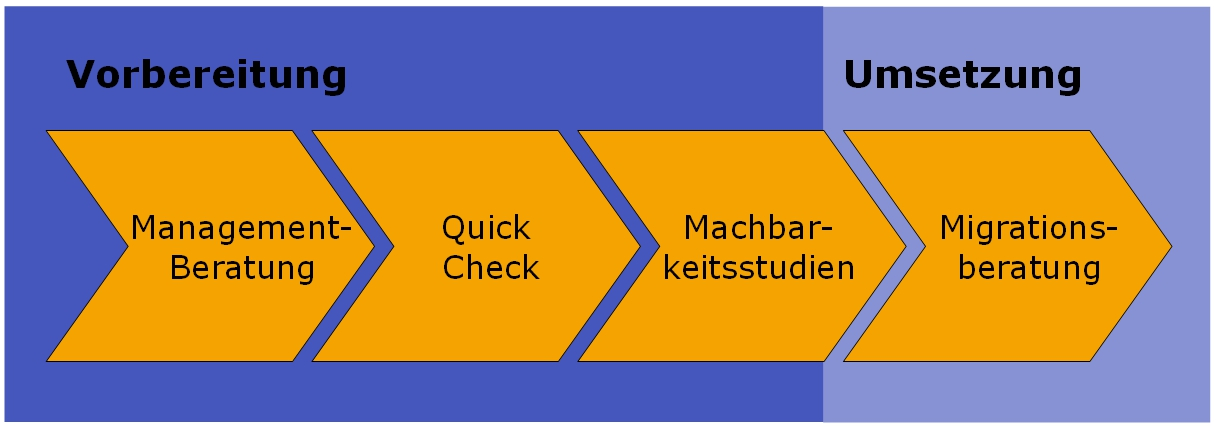
\includegraphics[width=6.5484in,height=1.9701in]{freiesoftwaredortmund-img2.png}
}

Darüber hinaus hat die Beauftragte der Bundesregierung für Informationstechnik
einen ``Leitfaden für die Migration von Software (Stand März
2012)''\footnote{\url{http://www.cio.bund.de/SharedDocs/Kurzmeldungen/DE/2012/20120305_migrationsleitfaden_4_0.html}
  [abgerufen am 16.03.2012]} herausgegeben.

\section{Schlusswort}

Für die städtische Umstellung auf OSS wird zu guter Letzt folgender schlicht
klingender, aber aussagekräftiger Arbeitstitel angeregt:

{\centering \textbf{DOSS -- Dortmunds Open Source Software}}

Abschließend eine persönliche Bemerkung: Unabhängigkeit von den Märkten ist
(besonders in diesen Tagen) ein unverzichtbarer Bestandteil verantwortlichen
Verwaltungshandelns.  Verwaltung muss agieren, statt nur zu reagieren. Der
skizzierte Lösungsvorschlag soll hierzu dienen!

\section{Lizenzhinweis}

{\centering 

\includegraphics[width=1.222in,height=0.4307in]{freiesoftwaredortmund-img3.png}
}


``Open Source Software im geschäftskritischen Einsatz bei der Stadt Dortmund''
erstellt am 30.04.2012 von Christian Nähle steht unter einer Creative Commons
Namensnennung-Weitergabe unter gleichen Bedingungen 3.0 Deutschland
Lizenz.\footnote{\url{http://creativecommons.org/licenses/by-sa/3.0/de/}
  [abgerufen am 09.04.2012]}

Der Autor ist per E-Mail erreichbar:
\href{mailto:c.naehle@gmx.net}{c.naehle@gmx.net}

Im Falle einer Verbreitung müssen Sie anderen alle Lizenzbedingungen mitteilen,
die für dieses Werk gelten. Dies stellt sicher, dass das in diesem Text
zusammengetragene Wissen von jeder Person stets frei vervielfältigt, kopiert,
verändert und somit für individuelle Ansprüche weiterentwickelt werden darf.


\includegraphics[width=0.6665in,height=0.6665in]{freiesoftwaredortmund-img4.png}
\emph{Namensnennung} -- Sie müssen den Namen des
Autors/Rechteinhabers in der von ihm festgelegten Weise nennen.


\includegraphics[width=0.6665in,height=0.6665in]{freiesoftwaredortmund-img5.png}
\emph{Weitergabe unter gleichen Bedingungen} -- Wenn
Sie das lizenzierte Werk bzw. den lizenzierten Inhalt bearbeiten oder
in anderer Weise erkennbar als Grundlage für eigenes Schaffen
verwenden, dürfen Sie die daraufhin neu entstandenen Werke bzw.
Inhalte nur unter Verwendung von Lizenzbedingungen weitergeben, die mit
denen dieses Lizenzvertrages identisch oder vergleichbar sind.

Danksagung

Ich danke Till Schäfer und Philipp Lewe dafür, dass sie mir Open Source Software
nächtelang auf meinem Balkon näher gebracht haben und mir hilfreich mit
Anmerkungen für den endlich vorliegenden Verbesserungsvorschlag für die Stadt
Dortmund zur Seite gestanden haben.

Gleichen Dank für wertvolle Anmerkungen schulde ich meinem Bruder Nicolai Parlog
und Church-of-Emacs-Anhänger Vlado Plaga.

Vor meiner Freundin und Lektorin, N. Fresen, verneige ich mich in tiefster
Dankbarkeit für ihre Unterstützung und ewige Geduld mit mir!

\section{Literaturliste}

{
{{Bundesverwaltungsamt: URL:
}}\href{http://www.bva.bund.de/}{{http://www.bva.bund.de}}
[abgerufen{{ am 22.03.2012]}}}

{
Bundesverwaltungsamt, Kompetenzzentrum Open Source Software: URL:
\href{https://www.oss.bund.de/node/107}{{http}}\href{https://www.oss.bund.de/node/107}{{s://www.oss.bund.de/node/107}}
{{[abgerufen am
13.03.2012]}}}

{
{Bundesverwaltungsamt, Kompetenzzentrum Open Source
Software: URL:
}\href{https://www.oss.bund.de/node/133}{{http}}\href{https://www.oss.bund.de/node/133}{{{s}}}\href{https://www.oss.bund.de/node/133}{{://www.oss.bund.de/node/133}}
{{[abgerufen am
13.03.2012]}}}

{
{{Bu}}{{ndesverwaltungsamt,
Kompetenzzentrum}}{ Open Source
Software}{{:
``Projekt LiMux in München''. URL:
}}\url{https://www.oss.bund.de/node/275}{{
}}{{[abgerufen am 13.03.2012]}}}

{
{{Creative Commons:
``Namensnennung-Weitergabe unter gleichen Bedingungen 3.0
Deutschland (CC BY-SA 3.0)''. URL:
}}\url{http://creativecommons.org/licenses/by-sa/3.0/de/}{{
[abgerufen am 09.04.2012]}}}


{
dosys -- IT-Konzept Stadt Dortmund 2011-2015, in der Stadtverwaltung
abgestimmter Entwurf; zur Vorlage im VV am 15.11.2011 und im Ausschuss
für Personal und Organisation am 22.11.11, Dortmund: Stadt Dortmund,
2011}

{
Ernst \& Young AG: ``Open Source Software im
geschäftskritischen Einsatz'', Broschüre, Ernst \&
Young AG, 2011}

{
{{Die Beauftragte der
Bundesregierung für Informationstechnik:
``Migrationsleitfaden in der Version 4.0
veröffentlicht''. URL:
}}\href{http://www.cio.bund.de/SharedDocs/Kurzmeldungen/DE/2012/20120305_migrationsleitfaden_4_0.html}{{http://www.cio.bund.de/SharedDocs/Kurzmeldungen/DE/2012/}}}

{
\href{http://www.cio.bund.de/SharedDocs/Kurzmeldungen/DE/2012/20120305_migrationsleitfaden_4_0.html}{{20120305\_migrationsleitfaden\_4\_0.html}}{{
[abgerufen am }}{{16.03.2012]}}}

{
{{Free Software Foundation Inc.:
``Was ist Freie Software?''. URL:
}}\url{http://www.gnu.org/philosophy/free-sw.de.html}{{
}}{{[abgerufen am 13.03.2012]}}}

{
GRüNE Ratsfraktion: ``Ergänzungsantrag zum IT-Konzept
2011-2015'', Dortmund, GRüNE Ratsfraktion,
08.02.2012}

{
Günther, Jochen Dipl.-Wi.-Ing: ``Open Source Software.
Strukturwandel oder Strohfeuer'' In: Spath, Dieter
Prof. Dr.-Ing (Hg.) ``Open Source Software. Strukturwandel
oder Strohfeuer'', Stuttgart: }

Fraunhofer Institut für Arbeitswirtschaft und Organisation, 2006

{
{{heise online:
``}}{{40.000}}{{
}}{{neue}}{{
}}{{Linux-Desktops}}{{
}}{{in}}{{
}}{{Spanien}}{{''}}{{.
URL:
}}\url{http://www.heise.de/open/meldung/40-000-neue-Linux-Desktops-in-Spanien-1419719.html}}

{
{{[abgerufen am 23.01.2012]}}}

{
{{heise online:
``}}{{Bundeswehr}}{{
}}{{setzt}}{{
}}{{auf}}{{
}}{{Open}}{{
}}{{Source}}{{
}}{{und}}{{
}}{{SOA}}{{''}}{{.
URL:
}}\href{http://www.heise.de/newsticker/meldung/Bundeswehr-setzt-auf-Open-Source-und-SOA-1430186.html}{{http://www.heise.de/newsticker/meldung/}}}

{
\href{http://www.heise.de/newsticker/meldung/Bundeswehr-setzt-auf-Open-Source-und-SOA-1430186.html}{{Bundeswehr-setzt-auf-Open-Source-und-SOA-1430186.html}}{{
}}{{[abgerufen am
07.02.2012]}}}

{
{{heise online:
``}}{{LiMux:}}{{
}}{{Billiger}}{{
}}{{und}}{{
}}{{robuster}}{{
}}{{als}}{{
}}{{Windows}}{{''}}{{.
URL:
}}\url{http://www.heise.de/open/meldung/LiMux-Billiger-und-robuster-als-Windows-1485410.html}}

{
{{[abgerufen am 07.04.2012]}}}

{
{{heise online:
``Niedersächsische Steuerverwaltung stellt auf Linux
um''. URL:
}}\href{http://www.heise.de/open/meldung/Niedersaechsische-Steuerverwaltung-stellt-auf-Linux-um-128541.html}{{http://www.heise.de/open/meldung/}}}

{
\href{http://www.heise.de/open/meldung/Niedersaechsische-Steuerverwaltung-stellt-auf-Linux-um-128541.html}{{Niedersaechsische-Steuerverwaltung-stellt-auf-Linux-um-128541.html}}{{
}}{[abgerufen am
}{{13.03.2012]}}}

{
{{heise online:
``}}{{Open}}{{
}}{{Source}}{{
}}{{für}}{{
}}{{New}}{{
}}{{Hampshire}}{{''}}{{.
URL:
}}\href{http://www.heise.de/open/meldung/Open-Source-fuer-New-Hampshire-1431833.html}{{http://www.heise.de/open/meldung/}}}

{
\href{http://www.heise.de/open/meldung/Open-Source-fuer-New-Hampshire-1431833.html}{{Open-Source-fuer-New-Hampshire-1431833.html}}{{
[abgerufen am 09.02.2012]}}}

{
{{heise online:
``Studie: Open-Source-Software qualitativ besser als
proprietäre Entwicklungen''. URL:
}}\url{http://heise.de/-1440788}{{
}}{{[abgerufen am
}}{{13.03.2012]}}}

{
{{Huber, Mathias (2012):
``}}{{Enterprise-Anwender}}{{
}}{{setzen}}{{
}}{{auf}}{{
}}{{Linux}}{{
}}{{für}}{{
}}{{Big}}{{
}}{{Data}}{{''.}}{{
}}}

{
{{URL:
}}\url{http://www.linux-magazin.de/NEWS/Enterprise-Anwender-setzen-auf-Linux-fuer-Big-Data}{{
}}{{[abgerufen am 15.03.2012]}}}

Kaczmarek, Oliver und andere Abgeordnete der SPD Bundestagsfraktion:
``Kleine Anfrage. Sachstand zur Nutzung von
{\quotesinglbase}freier Software{\textquoteleft} im Auswärtigen Amt
und weiteren Bundesbehörden.'' Elektronische
Vorabfassung, Berlin: H. Heenemann GmbH \& Co., 26.01.2011

{
{Kiefer,
Bernd}{{}-Uwe:}{
``}{FUM}{
}{08}{.
}{{Führungsaspekte}}{{
}}{{des}}{{
}}{{Projektmanagements}}{{''}}{{{.}}}{{{
}}}{{{Pfungstadt:}}}{{{
}}}{Studiengemeinschaft}{
}{Werner}{
}{Kamprath}{
}{Darmstadt}{
}{GmbH}{, 2012}}

{
{{Laufer, Simon (2011):
``}}{{20 Jahre
Linux}}{{{.
}}}{{Wie}}{{
}}{{der}}{{
}}{{Pinguin}}{{
}}{{nach}}{{
}}{{München}}{{
}}{{kam}}{{''.
URL:}}{{
}}\url{http://www.spiegel.de/netzwelt/web/0,1518,781680,00.html}
{{[abgerufen am 13.03.2012]}}}

{
{{{Norddeutscher
Rundfunk}}}{{:
``Deutschland bleibt IT-Mittelmaß''.
URL:
}}\url{http://www.tagesschau.de/inland/itgipfel120.html}{{
[abgerufen am 09.04.2012]}}}

{
{Renner,}{
}{Thomas}{
}{et}{
}{al.:}{
``}{Open}{
}{Source}{
}{Software}{.
}Einsparpotentiale und Wirtschaftlichkeit{\textquotedblright}.
Stuttgart: }

Fraunhofer Institut für Arbeitswirtschaft und Organisation, 2005

{
{{{Stadt}}}{{{
}}}{{{Dortmund}}}{{{
}}}{{{(Hg):}}}{{{
}}}{{``}}{{MAI}}{{{.}}}{{{
}}}{{Mitarbeiterinnen-}}{{
}}{{und}}{{
}}{{Mitarbeiterinformation}}{{{''}}}{{,}}{{
}}{{Nr.}}{{
}}{{3}}{{{/2011}}}{{,}}{{
}}{{{Dortmund:
Stadt Dortmund,
}}}{{2011,}}{{
}}{{S.}}{{
}}{{{6}}}}


{
{{Wikimedia}}{{
}}{{Foundation}}{{
}}{{Inc.:}}{{
``}}{{Datei:Opensource.svg}}{{''}}{{.}}{{
}}{{URL:}}{{
}}\url{https://de.wikipedia.org/w/index.php?title=Datei:Opensource.svg&filetimestamp=20070822051640}{{
}}{[abgerufen}{
}{am}{
}{13.03.2012]}}

{
{{Wikimedia Foundation Inc.:
``Digitale Kluft''. URL:
}}\url{https://de.wikipedia.org/wiki/Digitale_Kluft}{{
[abgerufen am 13.03.2012]}}}

{
{{Wikimedia Foundation Inc.:
``Kompilierung''. URL:
}}\url{https://de.wikipedia.org/wiki/Kompilierung}}

{
{{[abgerufen am 13.03.2012]}}}

{
{{Wikimedia Foundation Inc.:
``Know-how''. URL:
}}\url{https://de.wikipedia.org/wiki/Know-how}}

{
{{[abgerufen am 22.03.2012]}}}

{
{{Wikimedia Foundation Inc.:
``Offener Standard''.
URL:}}{{{
}}}\url{https://de.wikipedia.org/wiki/Offener_Standard}{{
}}{[abgerufen am 13.03.2012]}}

{
{{Wikimedia Foundation Inc.:
``Open Source''. URL:
}}\href{https://de.wikipedia.org/wiki/Open_Source#Begriffsproblem_.E2.80.9EFreie_Software.E2.80.9C
}{{https://de.wikipedia.org/wiki/Open\_Source\#Begriffsproblem\_.E2.80.9EFreie\_Software.E2.80.9C}}{{
[abgerufen am 13.03.2012]}}}

{
{{Wikimedia Foundation Inc.:
``Open-Source-Software in öffentlichen
Einrichtungen''.
URL:}}{{{
}}}\href{https://de.wikipedia.org/wiki/Open-Source-Software_in_?ffentlichen_Einrichtungen}{{https://de.wikipedia.org/wiki/Open-Source-Software\_in\_\%C3\%B6ffentlichen\_Einrichtungen}}}

{
{{[abgerufen am 05.03.2012]}}}

{
{{Wikimedia Foundation Inc.:
``Proprietäre Software''. URL:
}}\href{https://de.wikipedia.org/wiki/Propriet?re_Software}{{https://de.wikipedia.org/wiki/Propriet\%C3\%A4re\_Software}}{{
}}{[abgerufen am 13.03.2012]}}

{{{Wikimedia}}{{
}}{{Foundation}}{{
}}{{Inc.:}}{{
``}}{{Quelltext}}{{''}}{{.}}{{
}}{{URL:}}{{
}}\url{https://de.wikipedia.org/wiki/Quelltext}}

{[abgerufen am 07.04.2012]}

{
{{Wikimedia Foundation Inc.:
``Red Hat''. URL:
}}\url{https://de.wikipedia.org/wiki/Red_Hat}}

{
[abgerufen am 13.03.2012]}

{
{{Wikimedia Foundation Inc.:
``Softwarepatent''. URL:
}}\url{https://de.wikipedia.org/wiki/Softwarepatent#Europ.C3.A4ische_Union}}

{
[abgerufen am 16.03 2012]}

{
{{Wikimedia Foundation Inc.:
``Vier-Augen-Prinzip''. URL:
}}\href{https://de.wikipedia.org/wiki/Vier-Augen-Prinzip}{{https://de.wikipedia.org/wiki/}}}

{
\href{https://de.wikipedia.org/wiki/Vier-Augen-Prinzip}{{Vier-Augen-Prinzip}}{{
}}{[abgerufen am 13.03.2012]}}
\end{document}
